% Created by tikzDevice version 0.6.2 on 2012-04-22 09:19:32
% !TEX encoding = UTF-8 Unicode
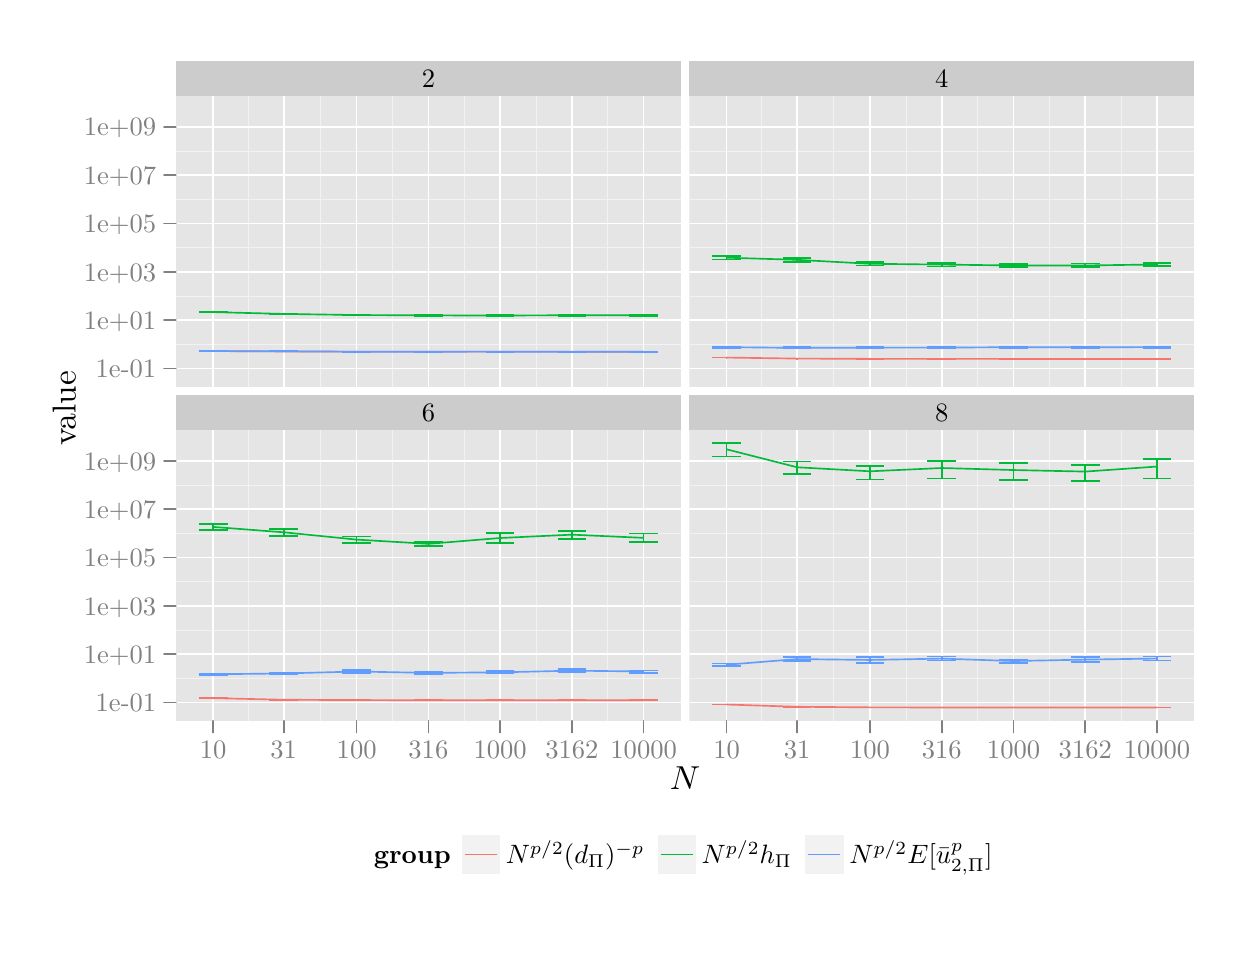
\begin{tikzpicture}[x=1pt,y=1pt]
\definecolor[named]{drawColor}{rgb}{0.00,0.00,0.00}
\definecolor[named]{fillColor}{rgb}{1.00,1.00,1.00}
\fill[color=fillColor,fill opacity=0.00,] (0,0) rectangle (433.62,325.21);
\begin{scope}
\path[clip] (  0.00,  0.00) rectangle (433.62,325.21);
\definecolor[named]{drawColor}{rgb}{0.41,0.16,0.58}
\end{scope}
\begin{scope}
\path[clip] (  0.00,  0.00) rectangle (433.62,325.21);
\definecolor[named]{drawColor}{rgb}{0.41,0.16,0.58}
\end{scope}
\begin{scope}
\path[clip] (  0.00,  0.00) rectangle (433.62,325.21);
\definecolor[named]{drawColor}{rgb}{0.41,0.16,0.58}
\end{scope}
\begin{scope}
\path[clip] (  0.00,  0.00) rectangle (433.62,325.21);
\definecolor[named]{drawColor}{rgb}{0.41,0.16,0.58}
\end{scope}
\begin{scope}
\path[clip] (  0.00,  0.00) rectangle (433.62,325.21);
\definecolor[named]{drawColor}{rgb}{0.41,0.16,0.58}
\end{scope}
\begin{scope}
\path[clip] (  0.00,  0.00) rectangle (433.62,325.21);
\definecolor[named]{drawColor}{rgb}{0.41,0.16,0.58}
\end{scope}
\begin{scope}
\path[clip] (  0.00,  0.00) rectangle (433.62,325.21);
\definecolor[named]{drawColor}{rgb}{0.41,0.16,0.58}
\end{scope}
\begin{scope}
\path[clip] (  0.00,  0.00) rectangle (433.62,325.21);
\definecolor[named]{drawColor}{rgb}{0.41,0.16,0.58}
\end{scope}
\begin{scope}
\path[clip] ( 53.55,195.47) rectangle (236.06,300.54);
\definecolor[named]{drawColor}{rgb}{0.41,0.16,0.58}
\end{scope}
\begin{scope}
\path[clip] (  0.00,  0.00) rectangle (433.62,325.21);
\definecolor[named]{drawColor}{rgb}{0.41,0.16,0.58}
\end{scope}
\begin{scope}
\path[clip] (239.07,195.47) rectangle (421.58,300.54);
\definecolor[named]{drawColor}{rgb}{0.41,0.16,0.58}
\end{scope}
\begin{scope}
\path[clip] (  0.00,  0.00) rectangle (433.62,325.21);
\definecolor[named]{drawColor}{rgb}{0.41,0.16,0.58}
\end{scope}
\begin{scope}
\path[clip] ( 53.55, 74.76) rectangle (236.06,179.83);
\definecolor[named]{drawColor}{rgb}{0.41,0.16,0.58}
\end{scope}
\begin{scope}
\path[clip] (  0.00,  0.00) rectangle (433.62,325.21);
\definecolor[named]{drawColor}{rgb}{0.41,0.16,0.58}
\end{scope}
\begin{scope}
\path[clip] (239.07, 74.76) rectangle (421.58,179.83);
\definecolor[named]{drawColor}{rgb}{0.41,0.16,0.58}
\end{scope}
\begin{scope}
\path[clip] (  0.00,  0.00) rectangle (433.62,325.21);
\definecolor[named]{drawColor}{rgb}{0.41,0.16,0.58}
\end{scope}
\begin{scope}
\path[clip] (  0.00,  0.00) rectangle (433.62,325.21);
\definecolor[named]{drawColor}{rgb}{0.41,0.16,0.58}
\end{scope}
\begin{scope}
\path[clip] (  0.00,  0.00) rectangle (433.62,325.21);
\definecolor[named]{drawColor}{rgb}{0.41,0.16,0.58}
\end{scope}
\begin{scope}
\path[clip] (  0.00,  0.00) rectangle (433.62,325.21);
\definecolor[named]{drawColor}{rgb}{0.41,0.16,0.58}
\end{scope}
\begin{scope}
\path[clip] (  0.00,  0.00) rectangle (433.62,325.21);
\definecolor[named]{drawColor}{rgb}{0.41,0.16,0.58}
\end{scope}
\begin{scope}
\path[clip] (  0.00,  0.00) rectangle (433.62,325.21);
\definecolor[named]{drawColor}{rgb}{0.41,0.16,0.58}
\end{scope}
\begin{scope}
\path[clip] (  0.00,  0.00) rectangle (433.62,325.21);
\definecolor[named]{drawColor}{rgb}{0.41,0.16,0.58}
\end{scope}
\begin{scope}
\path[clip] (  0.00,  0.00) rectangle (433.62,325.21);
\definecolor[named]{drawColor}{rgb}{0.41,0.16,0.58}
\end{scope}
\begin{scope}
\path[clip] (  0.00,  0.00) rectangle (433.62,325.21);
\definecolor[named]{drawColor}{rgb}{0.41,0.16,0.58}
\end{scope}
\begin{scope}
\path[clip] (  0.00,  0.00) rectangle (433.62,325.21);
\definecolor[named]{drawColor}{rgb}{0.41,0.16,0.58}
\end{scope}
\begin{scope}
\path[clip] (  0.00,  0.00) rectangle (433.62,325.21);
\definecolor[named]{drawColor}{rgb}{0.41,0.16,0.58}
\end{scope}
\begin{scope}
\path[clip] (  0.00,  0.00) rectangle (433.62,325.21);
\definecolor[named]{drawColor}{rgb}{0.41,0.16,0.58}
\end{scope}
\begin{scope}
\path[clip] (  0.00,  0.00) rectangle (433.62,325.21);
\definecolor[named]{drawColor}{rgb}{0.41,0.16,0.58}
\end{scope}
\begin{scope}
\path[clip] (  0.00,  0.00) rectangle (433.62,325.21);
\definecolor[named]{drawColor}{rgb}{0.41,0.16,0.58}
\end{scope}
\begin{scope}
\path[clip] (  0.00,  0.00) rectangle (433.62,325.21);
\definecolor[named]{drawColor}{rgb}{0.41,0.16,0.58}
\end{scope}
\begin{scope}
\path[clip] (  0.00,  0.00) rectangle (433.62,325.21);
\definecolor[named]{drawColor}{rgb}{0.41,0.16,0.58}
\end{scope}
\begin{scope}
\path[clip] (  0.00,  0.00) rectangle (433.62,325.21);
\definecolor[named]{drawColor}{rgb}{0.41,0.16,0.58}
\end{scope}
\begin{scope}
\path[clip] (  0.00,  0.00) rectangle (433.62,325.21);
\definecolor[named]{drawColor}{rgb}{0.41,0.16,0.58}
\end{scope}
\begin{scope}
\path[clip] (  0.00,  0.00) rectangle (433.62,325.21);
\definecolor[named]{drawColor}{rgb}{0.41,0.16,0.58}
\end{scope}
\begin{scope}
\path[clip] (  0.00,  0.00) rectangle (433.62,325.21);
\definecolor[named]{drawColor}{rgb}{0.41,0.16,0.58}
\end{scope}
\begin{scope}
\path[clip] (  0.00,  0.00) rectangle (433.62,325.21);
\definecolor[named]{drawColor}{rgb}{0.41,0.16,0.58}
\end{scope}
\begin{scope}
\path[clip] (  0.00,  0.00) rectangle (433.62,325.21);
\definecolor[named]{drawColor}{rgb}{0.41,0.16,0.58}
\end{scope}
\begin{scope}
\path[clip] (  0.00,  0.00) rectangle (433.62,325.21);
\definecolor[named]{drawColor}{rgb}{0.41,0.16,0.58}
\end{scope}
\begin{scope}
\path[clip] (  0.00,  0.00) rectangle (433.62,325.21);
\definecolor[named]{drawColor}{rgb}{0.41,0.16,0.58}
\end{scope}
\begin{scope}
\path[clip] (  0.00,  0.00) rectangle (433.62,325.21);
\definecolor[named]{drawColor}{rgb}{0.41,0.16,0.58}
\end{scope}
\begin{scope}
\path[clip] (  0.00,  0.00) rectangle (433.62,325.21);
\definecolor[named]{drawColor}{rgb}{0.41,0.16,0.58}
\end{scope}
\begin{scope}
\path[clip] (  0.00,  0.00) rectangle (433.62,325.21);
\definecolor[named]{drawColor}{rgb}{0.41,0.16,0.58}
\end{scope}
\begin{scope}
\path[clip] (  0.00,  0.00) rectangle (433.62,325.21);
\definecolor[named]{drawColor}{rgb}{0.41,0.16,0.58}
\end{scope}
\begin{scope}
\path[clip] (  0.00,  0.00) rectangle (433.62,325.21);
\definecolor[named]{drawColor}{rgb}{0.41,0.16,0.58}
\end{scope}
\begin{scope}
\path[clip] (  0.00,  0.00) rectangle (433.62,325.21);
\definecolor[named]{drawColor}{rgb}{0.41,0.16,0.58}
\end{scope}
\begin{scope}
\path[clip] (  0.00,  0.00) rectangle (433.62,325.21);
\definecolor[named]{drawColor}{rgb}{0.41,0.16,0.58}
\end{scope}
\begin{scope}
\path[clip] (  0.00,  0.00) rectangle (433.62,325.21);
\definecolor[named]{drawColor}{rgb}{0.41,0.16,0.58}
\end{scope}
\begin{scope}
\path[clip] (  0.00,  0.00) rectangle (433.62,325.21);
\definecolor[named]{drawColor}{rgb}{0.41,0.16,0.58}
\end{scope}
\begin{scope}
\path[clip] (  0.00,  0.00) rectangle (433.62,325.21);
\definecolor[named]{drawColor}{rgb}{0.41,0.16,0.58}
\definecolor[named]{fillColor}{rgb}{1.00,1.00,1.00}

\draw[fill=fillColor,draw opacity=0.00,] (  0.00,  0.00) rectangle (433.62,325.21);
\end{scope}
\begin{scope}
\path[clip] (  0.00,  0.00) rectangle (433.62,325.21);
\definecolor[named]{drawColor}{rgb}{0.41,0.16,0.58}
\end{scope}
\begin{scope}
\path[clip] ( 53.55,195.47) rectangle (236.06,300.54);
\definecolor[named]{drawColor}{rgb}{0.41,0.16,0.58}
\definecolor[named]{fillColor}{rgb}{0.90,0.90,0.90}

\draw[fill=fillColor,draw opacity=0.00,] ( 53.55,195.47) rectangle (236.06,300.54);
\definecolor[named]{drawColor}{rgb}{0.95,0.95,0.95}

\draw[color=drawColor,line width= 0.3pt,line cap=round,line join=round,fill opacity=0.00,] ( 53.55,210.76) --
	(236.06,210.76);

\draw[color=drawColor,line width= 0.3pt,line cap=round,line join=round,fill opacity=0.00,] ( 53.55,228.23) --
	(236.06,228.23);

\draw[color=drawColor,line width= 0.3pt,line cap=round,line join=round,fill opacity=0.00,] ( 53.55,245.70) --
	(236.06,245.70);

\draw[color=drawColor,line width= 0.3pt,line cap=round,line join=round,fill opacity=0.00,] ( 53.55,263.17) --
	(236.06,263.17);

\draw[color=drawColor,line width= 0.3pt,line cap=round,line join=round,fill opacity=0.00,] ( 53.55,280.64) --
	(236.06,280.64);

\draw[color=drawColor,line width= 0.3pt,line cap=round,line join=round,fill opacity=0.00,] ( 79.77,195.47) --
	( 79.77,300.54);

\draw[color=drawColor,line width= 0.3pt,line cap=round,line join=round,fill opacity=0.00,] (105.69,195.47) --
	(105.69,300.54);

\draw[color=drawColor,line width= 0.3pt,line cap=round,line join=round,fill opacity=0.00,] (131.83,195.47) --
	(131.83,300.54);

\draw[color=drawColor,line width= 0.3pt,line cap=round,line join=round,fill opacity=0.00,] (157.76,195.47) --
	(157.76,300.54);

\draw[color=drawColor,line width= 0.3pt,line cap=round,line join=round,fill opacity=0.00,] (183.69,195.47) --
	(183.69,300.54);

\draw[color=drawColor,line width= 0.3pt,line cap=round,line join=round,fill opacity=0.00,] (209.61,195.47) --
	(209.61,300.54);
\definecolor[named]{drawColor}{rgb}{1.00,1.00,1.00}

\draw[color=drawColor,line width= 0.6pt,line cap=round,line join=round,fill opacity=0.00,] ( 53.55,202.03) --
	(236.06,202.03);

\draw[color=drawColor,line width= 0.6pt,line cap=round,line join=round,fill opacity=0.00,] ( 53.55,219.50) --
	(236.06,219.50);

\draw[color=drawColor,line width= 0.6pt,line cap=round,line join=round,fill opacity=0.00,] ( 53.55,236.97) --
	(236.06,236.97);

\draw[color=drawColor,line width= 0.6pt,line cap=round,line join=round,fill opacity=0.00,] ( 53.55,254.44) --
	(236.06,254.44);

\draw[color=drawColor,line width= 0.6pt,line cap=round,line join=round,fill opacity=0.00,] ( 53.55,271.91) --
	(236.06,271.91);

\draw[color=drawColor,line width= 0.6pt,line cap=round,line join=round,fill opacity=0.00,] ( 53.55,289.38) --
	(236.06,289.38);

\draw[color=drawColor,line width= 0.6pt,line cap=round,line join=round,fill opacity=0.00,] ( 67.03,195.47) --
	( 67.03,300.54);

\draw[color=drawColor,line width= 0.6pt,line cap=round,line join=round,fill opacity=0.00,] ( 92.51,195.47) --
	( 92.51,300.54);

\draw[color=drawColor,line width= 0.6pt,line cap=round,line join=round,fill opacity=0.00,] (118.88,195.47) --
	(118.88,300.54);

\draw[color=drawColor,line width= 0.6pt,line cap=round,line join=round,fill opacity=0.00,] (144.79,195.47) --
	(144.79,300.54);

\draw[color=drawColor,line width= 0.6pt,line cap=round,line join=round,fill opacity=0.00,] (170.73,195.47) --
	(170.73,300.54);

\draw[color=drawColor,line width= 0.6pt,line cap=round,line join=round,fill opacity=0.00,] (196.65,195.47) --
	(196.65,300.54);

\draw[color=drawColor,line width= 0.6pt,line cap=round,line join=round,fill opacity=0.00,] (222.58,195.47) --
	(222.58,300.54);
\definecolor[named]{drawColor}{rgb}{0.97,0.46,0.43}

\draw[color=drawColor,line width= 0.6pt,line join=round,fill opacity=0.00,] ( 67.03,208.37) --
	( 92.51,208.20) --
	(118.88,208.15) --
	(144.79,208.14) --
	(170.73,208.14) --
	(196.65,208.13) --
	(222.58,208.13);
\definecolor[named]{drawColor}{rgb}{0.00,0.73,0.22}

\draw[color=drawColor,line width= 0.6pt,line join=round,fill opacity=0.00,] ( 67.03,222.43) --
	( 92.51,221.77) --
	(118.88,221.37) --
	(144.79,221.25) --
	(170.73,221.19) --
	(196.65,221.30) --
	(222.58,221.31);
\definecolor[named]{drawColor}{rgb}{0.38,0.61,1.00}

\draw[color=drawColor,line width= 0.6pt,line join=round,fill opacity=0.00,] ( 67.03,208.33) --
	( 92.51,208.25) --
	(118.88,208.12) --
	(144.79,208.12) --
	(170.73,208.14) --
	(196.65,208.07) --
	(222.58,208.14);
\definecolor[named]{drawColor}{rgb}{0.97,0.46,0.43}

\draw[color=drawColor,line width= 0.6pt,line join=round,fill opacity=0.00,] ( 61.85,208.37) --
	( 72.22,208.37);

\draw[color=drawColor,line width= 0.6pt,line join=round,fill opacity=0.00,] ( 67.03,208.37) --
	( 67.03,208.36);

\draw[color=drawColor,line width= 0.6pt,line join=round,fill opacity=0.00,] ( 61.85,208.36) --
	( 72.22,208.36);

\draw[color=drawColor,line width= 0.6pt,line join=round,fill opacity=0.00,] ( 87.32,208.20) --
	( 97.69,208.20);

\draw[color=drawColor,line width= 0.6pt,line join=round,fill opacity=0.00,] ( 92.51,208.20) --
	( 92.51,208.20);

\draw[color=drawColor,line width= 0.6pt,line join=round,fill opacity=0.00,] ( 87.32,208.20) --
	( 97.69,208.20);

\draw[color=drawColor,line width= 0.6pt,line join=round,fill opacity=0.00,] (113.69,208.15) --
	(124.06,208.15);

\draw[color=drawColor,line width= 0.6pt,line join=round,fill opacity=0.00,] (118.88,208.15) --
	(118.88,208.15);

\draw[color=drawColor,line width= 0.6pt,line join=round,fill opacity=0.00,] (113.69,208.15) --
	(124.06,208.15);

\draw[color=drawColor,line width= 0.6pt,line join=round,fill opacity=0.00,] (139.60,208.14) --
	(149.97,208.14);

\draw[color=drawColor,line width= 0.6pt,line join=round,fill opacity=0.00,] (144.79,208.14) --
	(144.79,208.14);

\draw[color=drawColor,line width= 0.6pt,line join=round,fill opacity=0.00,] (139.60,208.14) --
	(149.97,208.14);

\draw[color=drawColor,line width= 0.6pt,line join=round,fill opacity=0.00,] (165.54,208.14) --
	(175.91,208.14);

\draw[color=drawColor,line width= 0.6pt,line join=round,fill opacity=0.00,] (170.73,208.14) --
	(170.73,208.14);

\draw[color=drawColor,line width= 0.6pt,line join=round,fill opacity=0.00,] (165.54,208.14) --
	(175.91,208.14);

\draw[color=drawColor,line width= 0.6pt,line join=round,fill opacity=0.00,] (191.47,208.13) --
	(201.83,208.13);

\draw[color=drawColor,line width= 0.6pt,line join=round,fill opacity=0.00,] (196.65,208.13) --
	(196.65,208.13);

\draw[color=drawColor,line width= 0.6pt,line join=round,fill opacity=0.00,] (191.47,208.13) --
	(201.83,208.13);

\draw[color=drawColor,line width= 0.6pt,line join=round,fill opacity=0.00,] (217.39,208.13) --
	(227.76,208.13);

\draw[color=drawColor,line width= 0.6pt,line join=round,fill opacity=0.00,] (222.58,208.13) --
	(222.58,208.13);

\draw[color=drawColor,line width= 0.6pt,line join=round,fill opacity=0.00,] (217.39,208.13) --
	(227.76,208.13);
\definecolor[named]{drawColor}{rgb}{0.00,0.73,0.22}

\draw[color=drawColor,line width= 0.6pt,line join=round,fill opacity=0.00,] ( 61.85,222.60) --
	( 72.22,222.60);

\draw[color=drawColor,line width= 0.6pt,line join=round,fill opacity=0.00,] ( 67.03,222.60) --
	( 67.03,222.24);

\draw[color=drawColor,line width= 0.6pt,line join=round,fill opacity=0.00,] ( 61.85,222.24) --
	( 72.22,222.24);

\draw[color=drawColor,line width= 0.6pt,line join=round,fill opacity=0.00,] ( 87.32,221.97) --
	( 97.69,221.97);

\draw[color=drawColor,line width= 0.6pt,line join=round,fill opacity=0.00,] ( 92.51,221.97) --
	( 92.51,221.57);

\draw[color=drawColor,line width= 0.6pt,line join=round,fill opacity=0.00,] ( 87.32,221.57) --
	( 97.69,221.57);

\draw[color=drawColor,line width= 0.6pt,line join=round,fill opacity=0.00,] (113.69,221.57) --
	(124.06,221.57);

\draw[color=drawColor,line width= 0.6pt,line join=round,fill opacity=0.00,] (118.88,221.57) --
	(118.88,221.17);

\draw[color=drawColor,line width= 0.6pt,line join=round,fill opacity=0.00,] (113.69,221.17) --
	(124.06,221.17);

\draw[color=drawColor,line width= 0.6pt,line join=round,fill opacity=0.00,] (139.60,221.44) --
	(149.97,221.44);

\draw[color=drawColor,line width= 0.6pt,line join=round,fill opacity=0.00,] (144.79,221.44) --
	(144.79,221.05);

\draw[color=drawColor,line width= 0.6pt,line join=round,fill opacity=0.00,] (139.60,221.05) --
	(149.97,221.05);

\draw[color=drawColor,line width= 0.6pt,line join=round,fill opacity=0.00,] (165.54,221.38) --
	(175.91,221.38);

\draw[color=drawColor,line width= 0.6pt,line join=round,fill opacity=0.00,] (170.73,221.38) --
	(170.73,220.99);

\draw[color=drawColor,line width= 0.6pt,line join=round,fill opacity=0.00,] (165.54,220.99) --
	(175.91,220.99);

\draw[color=drawColor,line width= 0.6pt,line join=round,fill opacity=0.00,] (191.47,221.51) --
	(201.83,221.51);

\draw[color=drawColor,line width= 0.6pt,line join=round,fill opacity=0.00,] (196.65,221.51) --
	(196.65,221.12);

\draw[color=drawColor,line width= 0.6pt,line join=round,fill opacity=0.00,] (191.47,221.12) --
	(201.83,221.12);

\draw[color=drawColor,line width= 0.6pt,line join=round,fill opacity=0.00,] (217.39,221.51) --
	(227.76,221.51);

\draw[color=drawColor,line width= 0.6pt,line join=round,fill opacity=0.00,] (222.58,221.51) --
	(222.58,221.12);

\draw[color=drawColor,line width= 0.6pt,line join=round,fill opacity=0.00,] (217.39,221.12) --
	(227.76,221.12);
\definecolor[named]{drawColor}{rgb}{0.38,0.61,1.00}

\draw[color=drawColor,line width= 0.6pt,line join=round,fill opacity=0.00,] ( 61.85,208.43) --
	( 72.22,208.43);

\draw[color=drawColor,line width= 0.6pt,line join=round,fill opacity=0.00,] ( 67.03,208.43) --
	( 67.03,208.24);

\draw[color=drawColor,line width= 0.6pt,line join=round,fill opacity=0.00,] ( 61.85,208.24) --
	( 72.22,208.24);

\draw[color=drawColor,line width= 0.6pt,line join=round,fill opacity=0.00,] ( 87.32,208.36) --
	( 97.69,208.36);

\draw[color=drawColor,line width= 0.6pt,line join=round,fill opacity=0.00,] ( 92.51,208.36) --
	( 92.51,208.16);

\draw[color=drawColor,line width= 0.6pt,line join=round,fill opacity=0.00,] ( 87.32,208.16) --
	( 97.69,208.16);

\draw[color=drawColor,line width= 0.6pt,line join=round,fill opacity=0.00,] (113.69,208.22) --
	(124.06,208.22);

\draw[color=drawColor,line width= 0.6pt,line join=round,fill opacity=0.00,] (118.88,208.22) --
	(118.88,208.01);

\draw[color=drawColor,line width= 0.6pt,line join=round,fill opacity=0.00,] (113.69,208.01) --
	(124.06,208.01);

\draw[color=drawColor,line width= 0.6pt,line join=round,fill opacity=0.00,] (139.60,208.23) --
	(149.97,208.23);

\draw[color=drawColor,line width= 0.6pt,line join=round,fill opacity=0.00,] (144.79,208.23) --
	(144.79,208.01);

\draw[color=drawColor,line width= 0.6pt,line join=round,fill opacity=0.00,] (139.60,208.01) --
	(149.97,208.01);

\draw[color=drawColor,line width= 0.6pt,line join=round,fill opacity=0.00,] (165.54,208.25) --
	(175.91,208.25);

\draw[color=drawColor,line width= 0.6pt,line join=round,fill opacity=0.00,] (170.73,208.25) --
	(170.73,208.04);

\draw[color=drawColor,line width= 0.6pt,line join=round,fill opacity=0.00,] (165.54,208.04) --
	(175.91,208.04);

\draw[color=drawColor,line width= 0.6pt,line join=round,fill opacity=0.00,] (191.47,208.17) --
	(201.83,208.17);

\draw[color=drawColor,line width= 0.6pt,line join=round,fill opacity=0.00,] (196.65,208.17) --
	(196.65,207.97);

\draw[color=drawColor,line width= 0.6pt,line join=round,fill opacity=0.00,] (191.47,207.97) --
	(201.83,207.97);

\draw[color=drawColor,line width= 0.6pt,line join=round,fill opacity=0.00,] (217.39,208.25) --
	(227.76,208.25);

\draw[color=drawColor,line width= 0.6pt,line join=round,fill opacity=0.00,] (222.58,208.25) --
	(222.58,208.03);

\draw[color=drawColor,line width= 0.6pt,line join=round,fill opacity=0.00,] (217.39,208.03) --
	(227.76,208.03);
\end{scope}
\begin{scope}
\path[clip] (  0.00,  0.00) rectangle (433.62,325.21);
\definecolor[named]{drawColor}{rgb}{0.41,0.16,0.58}
\end{scope}
\begin{scope}
\path[clip] (239.07,195.47) rectangle (421.58,300.54);
\definecolor[named]{drawColor}{rgb}{0.41,0.16,0.58}
\definecolor[named]{fillColor}{rgb}{0.90,0.90,0.90}

\draw[fill=fillColor,draw opacity=0.00,] (239.07,195.47) rectangle (421.57,300.54);
\definecolor[named]{drawColor}{rgb}{0.95,0.95,0.95}

\draw[color=drawColor,line width= 0.3pt,line cap=round,line join=round,fill opacity=0.00,] (239.07,210.76) --
	(421.58,210.76);

\draw[color=drawColor,line width= 0.3pt,line cap=round,line join=round,fill opacity=0.00,] (239.07,228.23) --
	(421.58,228.23);

\draw[color=drawColor,line width= 0.3pt,line cap=round,line join=round,fill opacity=0.00,] (239.07,245.70) --
	(421.58,245.70);

\draw[color=drawColor,line width= 0.3pt,line cap=round,line join=round,fill opacity=0.00,] (239.07,263.17) --
	(421.58,263.17);

\draw[color=drawColor,line width= 0.3pt,line cap=round,line join=round,fill opacity=0.00,] (239.07,280.64) --
	(421.58,280.64);

\draw[color=drawColor,line width= 0.3pt,line cap=round,line join=round,fill opacity=0.00,] (265.29,195.47) --
	(265.29,300.54);

\draw[color=drawColor,line width= 0.3pt,line cap=round,line join=round,fill opacity=0.00,] (291.21,195.47) --
	(291.21,300.54);

\draw[color=drawColor,line width= 0.3pt,line cap=round,line join=round,fill opacity=0.00,] (317.35,195.47) --
	(317.35,300.54);

\draw[color=drawColor,line width= 0.3pt,line cap=round,line join=round,fill opacity=0.00,] (343.28,195.47) --
	(343.28,300.54);

\draw[color=drawColor,line width= 0.3pt,line cap=round,line join=round,fill opacity=0.00,] (369.21,195.47) --
	(369.21,300.54);

\draw[color=drawColor,line width= 0.3pt,line cap=round,line join=round,fill opacity=0.00,] (395.13,195.47) --
	(395.13,300.54);
\definecolor[named]{drawColor}{rgb}{1.00,1.00,1.00}

\draw[color=drawColor,line width= 0.6pt,line cap=round,line join=round,fill opacity=0.00,] (239.07,202.03) --
	(421.58,202.03);

\draw[color=drawColor,line width= 0.6pt,line cap=round,line join=round,fill opacity=0.00,] (239.07,219.50) --
	(421.58,219.50);

\draw[color=drawColor,line width= 0.6pt,line cap=round,line join=round,fill opacity=0.00,] (239.07,236.97) --
	(421.58,236.97);

\draw[color=drawColor,line width= 0.6pt,line cap=round,line join=round,fill opacity=0.00,] (239.07,254.44) --
	(421.58,254.44);

\draw[color=drawColor,line width= 0.6pt,line cap=round,line join=round,fill opacity=0.00,] (239.07,271.91) --
	(421.58,271.91);

\draw[color=drawColor,line width= 0.6pt,line cap=round,line join=round,fill opacity=0.00,] (239.07,289.38) --
	(421.58,289.38);

\draw[color=drawColor,line width= 0.6pt,line cap=round,line join=round,fill opacity=0.00,] (252.55,195.47) --
	(252.55,300.54);

\draw[color=drawColor,line width= 0.6pt,line cap=round,line join=round,fill opacity=0.00,] (278.03,195.47) --
	(278.03,300.54);

\draw[color=drawColor,line width= 0.6pt,line cap=round,line join=round,fill opacity=0.00,] (304.40,195.47) --
	(304.40,300.54);

\draw[color=drawColor,line width= 0.6pt,line cap=round,line join=round,fill opacity=0.00,] (330.31,195.47) --
	(330.31,300.54);

\draw[color=drawColor,line width= 0.6pt,line cap=round,line join=round,fill opacity=0.00,] (356.25,195.47) --
	(356.25,300.54);

\draw[color=drawColor,line width= 0.6pt,line cap=round,line join=round,fill opacity=0.00,] (382.17,195.47) --
	(382.17,300.54);

\draw[color=drawColor,line width= 0.6pt,line cap=round,line join=round,fill opacity=0.00,] (408.09,195.47) --
	(408.09,300.54);
\definecolor[named]{drawColor}{rgb}{0.97,0.46,0.43}

\draw[color=drawColor,line width= 0.6pt,line join=round,fill opacity=0.00,] (252.55,206.00) --
	(278.03,205.63) --
	(304.40,205.54) --
	(330.31,205.52) --
	(356.25,205.51) --
	(382.17,205.51) --
	(408.09,205.50);
\definecolor[named]{drawColor}{rgb}{0.00,0.73,0.22}

\draw[color=drawColor,line width= 0.6pt,line join=round,fill opacity=0.00,] (252.55,242.09) --
	(278.03,241.32) --
	(304.40,239.89) --
	(330.31,239.60) --
	(356.25,239.28) --
	(382.17,239.28) --
	(408.09,239.64);
\definecolor[named]{drawColor}{rgb}{0.38,0.61,1.00}

\draw[color=drawColor,line width= 0.6pt,line join=round,fill opacity=0.00,] (252.55,209.76) --
	(278.03,209.50) --
	(304.40,209.59) --
	(330.31,209.59) --
	(356.25,209.76) --
	(382.17,209.69) --
	(408.09,209.79);
\definecolor[named]{drawColor}{rgb}{0.97,0.46,0.43}

\draw[color=drawColor,line width= 0.6pt,line join=round,fill opacity=0.00,] (247.36,206.02) --
	(257.73,206.02);

\draw[color=drawColor,line width= 0.6pt,line join=round,fill opacity=0.00,] (252.55,206.02) --
	(252.55,205.98);

\draw[color=drawColor,line width= 0.6pt,line join=round,fill opacity=0.00,] (247.36,205.98) --
	(257.73,205.98);

\draw[color=drawColor,line width= 0.6pt,line join=round,fill opacity=0.00,] (272.84,205.64) --
	(283.21,205.64);

\draw[color=drawColor,line width= 0.6pt,line join=round,fill opacity=0.00,] (278.03,205.64) --
	(278.03,205.63);

\draw[color=drawColor,line width= 0.6pt,line join=round,fill opacity=0.00,] (272.84,205.63) --
	(283.21,205.63);

\draw[color=drawColor,line width= 0.6pt,line join=round,fill opacity=0.00,] (299.21,205.54) --
	(309.58,205.54);

\draw[color=drawColor,line width= 0.6pt,line join=round,fill opacity=0.00,] (304.40,205.54) --
	(304.40,205.54);

\draw[color=drawColor,line width= 0.6pt,line join=round,fill opacity=0.00,] (299.21,205.54) --
	(309.58,205.54);

\draw[color=drawColor,line width= 0.6pt,line join=round,fill opacity=0.00,] (325.12,205.52) --
	(335.49,205.52);

\draw[color=drawColor,line width= 0.6pt,line join=round,fill opacity=0.00,] (330.31,205.52) --
	(330.31,205.52);

\draw[color=drawColor,line width= 0.6pt,line join=round,fill opacity=0.00,] (325.12,205.52) --
	(335.49,205.52);

\draw[color=drawColor,line width= 0.6pt,line join=round,fill opacity=0.00,] (351.06,205.51) --
	(361.43,205.51);

\draw[color=drawColor,line width= 0.6pt,line join=round,fill opacity=0.00,] (356.25,205.51) --
	(356.25,205.51);

\draw[color=drawColor,line width= 0.6pt,line join=round,fill opacity=0.00,] (351.06,205.51) --
	(361.43,205.51);

\draw[color=drawColor,line width= 0.6pt,line join=round,fill opacity=0.00,] (376.98,205.51) --
	(387.35,205.51);

\draw[color=drawColor,line width= 0.6pt,line join=round,fill opacity=0.00,] (382.17,205.51) --
	(382.17,205.51);

\draw[color=drawColor,line width= 0.6pt,line join=round,fill opacity=0.00,] (376.98,205.51) --
	(387.35,205.51);

\draw[color=drawColor,line width= 0.6pt,line join=round,fill opacity=0.00,] (402.91,205.50) --
	(413.28,205.50);

\draw[color=drawColor,line width= 0.6pt,line join=round,fill opacity=0.00,] (408.09,205.50) --
	(408.09,205.50);

\draw[color=drawColor,line width= 0.6pt,line join=round,fill opacity=0.00,] (402.91,205.50) --
	(413.28,205.50);
\definecolor[named]{drawColor}{rgb}{0.00,0.73,0.22}

\draw[color=drawColor,line width= 0.6pt,line join=round,fill opacity=0.00,] (247.36,242.67) --
	(257.73,242.67);

\draw[color=drawColor,line width= 0.6pt,line join=round,fill opacity=0.00,] (252.55,242.67) --
	(252.55,241.48);

\draw[color=drawColor,line width= 0.6pt,line join=round,fill opacity=0.00,] (247.36,241.48) --
	(257.73,241.48);

\draw[color=drawColor,line width= 0.6pt,line join=round,fill opacity=0.00,] (272.84,241.97) --
	(283.21,241.97);

\draw[color=drawColor,line width= 0.6pt,line join=round,fill opacity=0.00,] (278.03,241.97) --
	(278.03,240.59);

\draw[color=drawColor,line width= 0.6pt,line join=round,fill opacity=0.00,] (272.84,240.59) --
	(283.21,240.59);

\draw[color=drawColor,line width= 0.6pt,line join=round,fill opacity=0.00,] (299.21,240.50) --
	(309.58,240.50);

\draw[color=drawColor,line width= 0.6pt,line join=round,fill opacity=0.00,] (304.40,240.50) --
	(304.40,239.24);

\draw[color=drawColor,line width= 0.6pt,line join=round,fill opacity=0.00,] (299.21,239.24) --
	(309.58,239.24);

\draw[color=drawColor,line width= 0.6pt,line join=round,fill opacity=0.00,] (325.12,240.29) --
	(335.49,240.29);

\draw[color=drawColor,line width= 0.6pt,line join=round,fill opacity=0.00,] (330.31,240.29) --
	(330.31,238.89);

\draw[color=drawColor,line width= 0.6pt,line join=round,fill opacity=0.00,] (325.12,238.89) --
	(335.49,238.89);

\draw[color=drawColor,line width= 0.6pt,line join=round,fill opacity=0.00,] (351.06,239.79) --
	(361.43,239.79);

\draw[color=drawColor,line width= 0.6pt,line join=round,fill opacity=0.00,] (356.25,239.79) --
	(356.25,238.70);

\draw[color=drawColor,line width= 0.6pt,line join=round,fill opacity=0.00,] (351.06,238.70) --
	(361.43,238.70);

\draw[color=drawColor,line width= 0.6pt,line join=round,fill opacity=0.00,] (376.98,239.93) --
	(387.35,239.93);

\draw[color=drawColor,line width= 0.6pt,line join=round,fill opacity=0.00,] (382.17,239.93) --
	(382.17,238.62);

\draw[color=drawColor,line width= 0.6pt,line join=round,fill opacity=0.00,] (376.98,238.62) --
	(387.35,238.62);

\draw[color=drawColor,line width= 0.6pt,line join=round,fill opacity=0.00,] (402.91,240.24) --
	(413.28,240.24);

\draw[color=drawColor,line width= 0.6pt,line join=round,fill opacity=0.00,] (408.09,240.24) --
	(408.09,239.07);

\draw[color=drawColor,line width= 0.6pt,line join=round,fill opacity=0.00,] (402.91,239.07) --
	(413.28,239.07);
\definecolor[named]{drawColor}{rgb}{0.38,0.61,1.00}

\draw[color=drawColor,line width= 0.6pt,line join=round,fill opacity=0.00,] (247.36,209.96) --
	(257.73,209.96);

\draw[color=drawColor,line width= 0.6pt,line join=round,fill opacity=0.00,] (252.55,209.96) --
	(252.55,209.56);

\draw[color=drawColor,line width= 0.6pt,line join=round,fill opacity=0.00,] (247.36,209.56) --
	(257.73,209.56);

\draw[color=drawColor,line width= 0.6pt,line join=round,fill opacity=0.00,] (272.84,209.71) --
	(283.21,209.71);

\draw[color=drawColor,line width= 0.6pt,line join=round,fill opacity=0.00,] (278.03,209.71) --
	(278.03,209.24);

\draw[color=drawColor,line width= 0.6pt,line join=round,fill opacity=0.00,] (272.84,209.24) --
	(283.21,209.24);

\draw[color=drawColor,line width= 0.6pt,line join=round,fill opacity=0.00,] (299.21,209.83) --
	(309.58,209.83);

\draw[color=drawColor,line width= 0.6pt,line join=round,fill opacity=0.00,] (304.40,209.83) --
	(304.40,209.35);

\draw[color=drawColor,line width= 0.6pt,line join=round,fill opacity=0.00,] (299.21,209.35) --
	(309.58,209.35);

\draw[color=drawColor,line width= 0.6pt,line join=round,fill opacity=0.00,] (325.12,209.83) --
	(335.49,209.83);

\draw[color=drawColor,line width= 0.6pt,line join=round,fill opacity=0.00,] (330.31,209.83) --
	(330.31,209.35);

\draw[color=drawColor,line width= 0.6pt,line join=round,fill opacity=0.00,] (325.12,209.35) --
	(335.49,209.35);

\draw[color=drawColor,line width= 0.6pt,line join=round,fill opacity=0.00,] (351.06,209.99) --
	(361.43,209.99);

\draw[color=drawColor,line width= 0.6pt,line join=round,fill opacity=0.00,] (356.25,209.99) --
	(356.25,209.52);

\draw[color=drawColor,line width= 0.6pt,line join=round,fill opacity=0.00,] (351.06,209.52) --
	(361.43,209.52);

\draw[color=drawColor,line width= 0.6pt,line join=round,fill opacity=0.00,] (376.98,209.93) --
	(387.35,209.93);

\draw[color=drawColor,line width= 0.6pt,line join=round,fill opacity=0.00,] (382.17,209.93) --
	(382.17,209.44);

\draw[color=drawColor,line width= 0.6pt,line join=round,fill opacity=0.00,] (376.98,209.44) --
	(387.35,209.44);

\draw[color=drawColor,line width= 0.6pt,line join=round,fill opacity=0.00,] (402.91,210.01) --
	(413.28,210.01);

\draw[color=drawColor,line width= 0.6pt,line join=round,fill opacity=0.00,] (408.09,210.01) --
	(408.09,209.52);

\draw[color=drawColor,line width= 0.6pt,line join=round,fill opacity=0.00,] (402.91,209.52) --
	(413.28,209.52);
\end{scope}
\begin{scope}
\path[clip] (  0.00,  0.00) rectangle (433.62,325.21);
\definecolor[named]{drawColor}{rgb}{0.41,0.16,0.58}
\end{scope}
\begin{scope}
\path[clip] ( 53.55, 74.76) rectangle (236.06,179.83);
\definecolor[named]{drawColor}{rgb}{0.41,0.16,0.58}
\definecolor[named]{fillColor}{rgb}{0.90,0.90,0.90}

\draw[fill=fillColor,draw opacity=0.00,] ( 53.55, 74.76) rectangle (236.06,179.83);
\definecolor[named]{drawColor}{rgb}{0.95,0.95,0.95}

\draw[color=drawColor,line width= 0.3pt,line cap=round,line join=round,fill opacity=0.00,] ( 53.55, 90.05) --
	(236.06, 90.05);

\draw[color=drawColor,line width= 0.3pt,line cap=round,line join=round,fill opacity=0.00,] ( 53.55,107.52) --
	(236.06,107.52);

\draw[color=drawColor,line width= 0.3pt,line cap=round,line join=round,fill opacity=0.00,] ( 53.55,124.99) --
	(236.06,124.99);

\draw[color=drawColor,line width= 0.3pt,line cap=round,line join=round,fill opacity=0.00,] ( 53.55,142.46) --
	(236.06,142.46);

\draw[color=drawColor,line width= 0.3pt,line cap=round,line join=round,fill opacity=0.00,] ( 53.55,159.93) --
	(236.06,159.93);

\draw[color=drawColor,line width= 0.3pt,line cap=round,line join=round,fill opacity=0.00,] ( 79.77, 74.76) --
	( 79.77,179.83);

\draw[color=drawColor,line width= 0.3pt,line cap=round,line join=round,fill opacity=0.00,] (105.69, 74.76) --
	(105.69,179.83);

\draw[color=drawColor,line width= 0.3pt,line cap=round,line join=round,fill opacity=0.00,] (131.83, 74.76) --
	(131.83,179.83);

\draw[color=drawColor,line width= 0.3pt,line cap=round,line join=round,fill opacity=0.00,] (157.76, 74.76) --
	(157.76,179.83);

\draw[color=drawColor,line width= 0.3pt,line cap=round,line join=round,fill opacity=0.00,] (183.69, 74.76) --
	(183.69,179.83);

\draw[color=drawColor,line width= 0.3pt,line cap=round,line join=round,fill opacity=0.00,] (209.61, 74.76) --
	(209.61,179.83);
\definecolor[named]{drawColor}{rgb}{1.00,1.00,1.00}

\draw[color=drawColor,line width= 0.6pt,line cap=round,line join=round,fill opacity=0.00,] ( 53.55, 81.32) --
	(236.06, 81.32);

\draw[color=drawColor,line width= 0.6pt,line cap=round,line join=round,fill opacity=0.00,] ( 53.55, 98.79) --
	(236.06, 98.79);

\draw[color=drawColor,line width= 0.6pt,line cap=round,line join=round,fill opacity=0.00,] ( 53.55,116.26) --
	(236.06,116.26);

\draw[color=drawColor,line width= 0.6pt,line cap=round,line join=round,fill opacity=0.00,] ( 53.55,133.73) --
	(236.06,133.73);

\draw[color=drawColor,line width= 0.6pt,line cap=round,line join=round,fill opacity=0.00,] ( 53.55,151.20) --
	(236.06,151.20);

\draw[color=drawColor,line width= 0.6pt,line cap=round,line join=round,fill opacity=0.00,] ( 53.55,168.67) --
	(236.06,168.67);

\draw[color=drawColor,line width= 0.6pt,line cap=round,line join=round,fill opacity=0.00,] ( 67.03, 74.76) --
	( 67.03,179.83);

\draw[color=drawColor,line width= 0.6pt,line cap=round,line join=round,fill opacity=0.00,] ( 92.51, 74.76) --
	( 92.51,179.83);

\draw[color=drawColor,line width= 0.6pt,line cap=round,line join=round,fill opacity=0.00,] (118.88, 74.76) --
	(118.88,179.83);

\draw[color=drawColor,line width= 0.6pt,line cap=round,line join=round,fill opacity=0.00,] (144.79, 74.76) --
	(144.79,179.83);

\draw[color=drawColor,line width= 0.6pt,line cap=round,line join=round,fill opacity=0.00,] (170.73, 74.76) --
	(170.73,179.83);

\draw[color=drawColor,line width= 0.6pt,line cap=round,line join=round,fill opacity=0.00,] (196.65, 74.76) --
	(196.65,179.83);

\draw[color=drawColor,line width= 0.6pt,line cap=round,line join=round,fill opacity=0.00,] (222.58, 74.76) --
	(222.58,179.83);
\definecolor[named]{drawColor}{rgb}{0.97,0.46,0.43}

\draw[color=drawColor,line width= 0.6pt,line join=round,fill opacity=0.00,] ( 67.03, 82.93) --
	( 92.51, 82.36) --
	(118.88, 82.22) --
	(144.79, 82.18) --
	(170.73, 82.17) --
	(196.65, 82.17) --
	(222.58, 82.16);
\definecolor[named]{drawColor}{rgb}{0.00,0.73,0.22}

\draw[color=drawColor,line width= 0.6pt,line join=round,fill opacity=0.00,] ( 67.03,144.80) --
	( 92.51,142.86) --
	(118.88,140.22) --
	(144.79,138.69) --
	(170.73,140.80) --
	(196.65,142.01) --
	(222.58,140.85);
\definecolor[named]{drawColor}{rgb}{0.38,0.61,1.00}

\draw[color=drawColor,line width= 0.6pt,line join=round,fill opacity=0.00,] ( 67.03, 91.57) --
	( 92.51, 91.85) --
	(118.88, 92.56) --
	(144.79, 92.06) --
	(170.73, 92.26) --
	(196.65, 92.86) --
	(222.58, 92.57);
\definecolor[named]{drawColor}{rgb}{0.97,0.46,0.43}

\draw[color=drawColor,line width= 0.6pt,line join=round,fill opacity=0.00,] ( 61.85, 82.96) --
	( 72.22, 82.96);

\draw[color=drawColor,line width= 0.6pt,line join=round,fill opacity=0.00,] ( 67.03, 82.96) --
	( 67.03, 82.91);

\draw[color=drawColor,line width= 0.6pt,line join=round,fill opacity=0.00,] ( 61.85, 82.91) --
	( 72.22, 82.91);

\draw[color=drawColor,line width= 0.6pt,line join=round,fill opacity=0.00,] ( 87.32, 82.36) --
	( 97.69, 82.36);

\draw[color=drawColor,line width= 0.6pt,line join=round,fill opacity=0.00,] ( 92.51, 82.36) --
	( 92.51, 82.35);

\draw[color=drawColor,line width= 0.6pt,line join=round,fill opacity=0.00,] ( 87.32, 82.35) --
	( 97.69, 82.35);

\draw[color=drawColor,line width= 0.6pt,line join=round,fill opacity=0.00,] (113.69, 82.23) --
	(124.06, 82.23);

\draw[color=drawColor,line width= 0.6pt,line join=round,fill opacity=0.00,] (118.88, 82.23) --
	(118.88, 82.22);

\draw[color=drawColor,line width= 0.6pt,line join=round,fill opacity=0.00,] (113.69, 82.22) --
	(124.06, 82.22);

\draw[color=drawColor,line width= 0.6pt,line join=round,fill opacity=0.00,] (139.60, 82.18) --
	(149.97, 82.18);

\draw[color=drawColor,line width= 0.6pt,line join=round,fill opacity=0.00,] (144.79, 82.18) --
	(144.79, 82.18);

\draw[color=drawColor,line width= 0.6pt,line join=round,fill opacity=0.00,] (139.60, 82.18) --
	(149.97, 82.18);

\draw[color=drawColor,line width= 0.6pt,line join=round,fill opacity=0.00,] (165.54, 82.17) --
	(175.91, 82.17);

\draw[color=drawColor,line width= 0.6pt,line join=round,fill opacity=0.00,] (170.73, 82.17) --
	(170.73, 82.17);

\draw[color=drawColor,line width= 0.6pt,line join=round,fill opacity=0.00,] (165.54, 82.17) --
	(175.91, 82.17);

\draw[color=drawColor,line width= 0.6pt,line join=round,fill opacity=0.00,] (191.47, 82.17) --
	(201.83, 82.17);

\draw[color=drawColor,line width= 0.6pt,line join=round,fill opacity=0.00,] (196.65, 82.17) --
	(196.65, 82.17);

\draw[color=drawColor,line width= 0.6pt,line join=round,fill opacity=0.00,] (191.47, 82.17) --
	(201.83, 82.17);

\draw[color=drawColor,line width= 0.6pt,line join=round,fill opacity=0.00,] (217.39, 82.16) --
	(227.76, 82.16);

\draw[color=drawColor,line width= 0.6pt,line join=round,fill opacity=0.00,] (222.58, 82.16) --
	(222.58, 82.16);

\draw[color=drawColor,line width= 0.6pt,line join=round,fill opacity=0.00,] (217.39, 82.16) --
	(227.76, 82.16);
\definecolor[named]{drawColor}{rgb}{0.00,0.73,0.22}

\draw[color=drawColor,line width= 0.6pt,line join=round,fill opacity=0.00,] ( 61.85,145.85) --
	( 72.22,145.85);

\draw[color=drawColor,line width= 0.6pt,line join=round,fill opacity=0.00,] ( 67.03,145.85) --
	( 67.03,143.60);

\draw[color=drawColor,line width= 0.6pt,line join=round,fill opacity=0.00,] ( 61.85,143.60) --
	( 72.22,143.60);

\draw[color=drawColor,line width= 0.6pt,line join=round,fill opacity=0.00,] ( 87.32,144.13) --
	( 97.69,144.13);

\draw[color=drawColor,line width= 0.6pt,line join=round,fill opacity=0.00,] ( 92.51,144.13) --
	( 92.51,141.44);

\draw[color=drawColor,line width= 0.6pt,line join=round,fill opacity=0.00,] ( 87.32,141.44) --
	( 97.69,141.44);

\draw[color=drawColor,line width= 0.6pt,line join=round,fill opacity=0.00,] (113.69,141.36) --
	(124.06,141.36);

\draw[color=drawColor,line width= 0.6pt,line join=round,fill opacity=0.00,] (118.88,141.36) --
	(118.88,138.93);

\draw[color=drawColor,line width= 0.6pt,line join=round,fill opacity=0.00,] (113.69,138.93) --
	(124.06,138.93);

\draw[color=drawColor,line width= 0.6pt,line join=round,fill opacity=0.00,] (139.60,139.46) --
	(149.97,139.46);

\draw[color=drawColor,line width= 0.6pt,line join=round,fill opacity=0.00,] (144.79,139.46) --
	(144.79,137.83);

\draw[color=drawColor,line width= 0.6pt,line join=round,fill opacity=0.00,] (139.60,137.83) --
	(149.97,137.83);

\draw[color=drawColor,line width= 0.6pt,line join=round,fill opacity=0.00,] (165.54,142.62) --
	(175.91,142.62);

\draw[color=drawColor,line width= 0.6pt,line join=round,fill opacity=0.00,] (170.73,142.62) --
	(170.73,138.95);

\draw[color=drawColor,line width= 0.6pt,line join=round,fill opacity=0.00,] (165.54,138.95) --
	(175.91,138.95);

\draw[color=drawColor,line width= 0.6pt,line join=round,fill opacity=0.00,] (191.47,143.42) --
	(201.83,143.42);

\draw[color=drawColor,line width= 0.6pt,line join=round,fill opacity=0.00,] (196.65,143.42) --
	(196.65,140.48);

\draw[color=drawColor,line width= 0.6pt,line join=round,fill opacity=0.00,] (191.47,140.48) --
	(201.83,140.48);

\draw[color=drawColor,line width= 0.6pt,line join=round,fill opacity=0.00,] (217.39,142.38) --
	(227.76,142.38);

\draw[color=drawColor,line width= 0.6pt,line join=round,fill opacity=0.00,] (222.58,142.38) --
	(222.58,139.28);

\draw[color=drawColor,line width= 0.6pt,line join=round,fill opacity=0.00,] (217.39,139.28) --
	(227.76,139.28);
\definecolor[named]{drawColor}{rgb}{0.38,0.61,1.00}

\draw[color=drawColor,line width= 0.6pt,line join=round,fill opacity=0.00,] ( 61.85, 91.87) --
	( 72.22, 91.87);

\draw[color=drawColor,line width= 0.6pt,line join=round,fill opacity=0.00,] ( 67.03, 91.87) --
	( 67.03, 91.27);

\draw[color=drawColor,line width= 0.6pt,line join=round,fill opacity=0.00,] ( 61.85, 91.27) --
	( 72.22, 91.27);

\draw[color=drawColor,line width= 0.6pt,line join=round,fill opacity=0.00,] ( 87.32, 92.26) --
	( 97.69, 92.26);

\draw[color=drawColor,line width= 0.6pt,line join=round,fill opacity=0.00,] ( 92.51, 92.26) --
	( 92.51, 91.42);

\draw[color=drawColor,line width= 0.6pt,line join=round,fill opacity=0.00,] ( 87.32, 91.42) --
	( 97.69, 91.42);

\draw[color=drawColor,line width= 0.6pt,line join=round,fill opacity=0.00,] (113.69, 93.13) --
	(124.06, 93.13);

\draw[color=drawColor,line width= 0.6pt,line join=round,fill opacity=0.00,] (118.88, 93.13) --
	(118.88, 91.99);

\draw[color=drawColor,line width= 0.6pt,line join=round,fill opacity=0.00,] (113.69, 91.99) --
	(124.06, 91.99);

\draw[color=drawColor,line width= 0.6pt,line join=round,fill opacity=0.00,] (139.60, 92.55) --
	(149.97, 92.55);

\draw[color=drawColor,line width= 0.6pt,line join=round,fill opacity=0.00,] (144.79, 92.55) --
	(144.79, 91.55);

\draw[color=drawColor,line width= 0.6pt,line join=round,fill opacity=0.00,] (139.60, 91.55) --
	(149.97, 91.55);

\draw[color=drawColor,line width= 0.6pt,line join=round,fill opacity=0.00,] (165.54, 92.70) --
	(175.91, 92.70);

\draw[color=drawColor,line width= 0.6pt,line join=round,fill opacity=0.00,] (170.73, 92.70) --
	(170.73, 91.78);

\draw[color=drawColor,line width= 0.6pt,line join=round,fill opacity=0.00,] (165.54, 91.78) --
	(175.91, 91.78);

\draw[color=drawColor,line width= 0.6pt,line join=round,fill opacity=0.00,] (191.47, 93.38) --
	(201.83, 93.38);

\draw[color=drawColor,line width= 0.6pt,line join=round,fill opacity=0.00,] (196.65, 93.38) --
	(196.65, 92.35);

\draw[color=drawColor,line width= 0.6pt,line join=round,fill opacity=0.00,] (191.47, 92.35) --
	(201.83, 92.35);

\draw[color=drawColor,line width= 0.6pt,line join=round,fill opacity=0.00,] (217.39, 92.98) --
	(227.76, 92.98);

\draw[color=drawColor,line width= 0.6pt,line join=round,fill opacity=0.00,] (222.58, 92.98) --
	(222.58, 92.12);

\draw[color=drawColor,line width= 0.6pt,line join=round,fill opacity=0.00,] (217.39, 92.12) --
	(227.76, 92.12);
\end{scope}
\begin{scope}
\path[clip] (  0.00,  0.00) rectangle (433.62,325.21);
\definecolor[named]{drawColor}{rgb}{0.41,0.16,0.58}
\end{scope}
\begin{scope}
\path[clip] (239.07, 74.76) rectangle (421.58,179.83);
\definecolor[named]{drawColor}{rgb}{0.41,0.16,0.58}
\definecolor[named]{fillColor}{rgb}{0.90,0.90,0.90}

\draw[fill=fillColor,draw opacity=0.00,] (239.07, 74.76) rectangle (421.57,179.83);
\definecolor[named]{drawColor}{rgb}{0.95,0.95,0.95}

\draw[color=drawColor,line width= 0.3pt,line cap=round,line join=round,fill opacity=0.00,] (239.07, 90.05) --
	(421.58, 90.05);

\draw[color=drawColor,line width= 0.3pt,line cap=round,line join=round,fill opacity=0.00,] (239.07,107.52) --
	(421.58,107.52);

\draw[color=drawColor,line width= 0.3pt,line cap=round,line join=round,fill opacity=0.00,] (239.07,124.99) --
	(421.58,124.99);

\draw[color=drawColor,line width= 0.3pt,line cap=round,line join=round,fill opacity=0.00,] (239.07,142.46) --
	(421.58,142.46);

\draw[color=drawColor,line width= 0.3pt,line cap=round,line join=round,fill opacity=0.00,] (239.07,159.93) --
	(421.58,159.93);

\draw[color=drawColor,line width= 0.3pt,line cap=round,line join=round,fill opacity=0.00,] (265.29, 74.76) --
	(265.29,179.83);

\draw[color=drawColor,line width= 0.3pt,line cap=round,line join=round,fill opacity=0.00,] (291.21, 74.76) --
	(291.21,179.83);

\draw[color=drawColor,line width= 0.3pt,line cap=round,line join=round,fill opacity=0.00,] (317.35, 74.76) --
	(317.35,179.83);

\draw[color=drawColor,line width= 0.3pt,line cap=round,line join=round,fill opacity=0.00,] (343.28, 74.76) --
	(343.28,179.83);

\draw[color=drawColor,line width= 0.3pt,line cap=round,line join=round,fill opacity=0.00,] (369.21, 74.76) --
	(369.21,179.83);

\draw[color=drawColor,line width= 0.3pt,line cap=round,line join=round,fill opacity=0.00,] (395.13, 74.76) --
	(395.13,179.83);
\definecolor[named]{drawColor}{rgb}{1.00,1.00,1.00}

\draw[color=drawColor,line width= 0.6pt,line cap=round,line join=round,fill opacity=0.00,] (239.07, 81.32) --
	(421.58, 81.32);

\draw[color=drawColor,line width= 0.6pt,line cap=round,line join=round,fill opacity=0.00,] (239.07, 98.79) --
	(421.58, 98.79);

\draw[color=drawColor,line width= 0.6pt,line cap=round,line join=round,fill opacity=0.00,] (239.07,116.26) --
	(421.58,116.26);

\draw[color=drawColor,line width= 0.6pt,line cap=round,line join=round,fill opacity=0.00,] (239.07,133.73) --
	(421.58,133.73);

\draw[color=drawColor,line width= 0.6pt,line cap=round,line join=round,fill opacity=0.00,] (239.07,151.20) --
	(421.58,151.20);

\draw[color=drawColor,line width= 0.6pt,line cap=round,line join=round,fill opacity=0.00,] (239.07,168.67) --
	(421.58,168.67);

\draw[color=drawColor,line width= 0.6pt,line cap=round,line join=round,fill opacity=0.00,] (252.55, 74.76) --
	(252.55,179.83);

\draw[color=drawColor,line width= 0.6pt,line cap=round,line join=round,fill opacity=0.00,] (278.03, 74.76) --
	(278.03,179.83);

\draw[color=drawColor,line width= 0.6pt,line cap=round,line join=round,fill opacity=0.00,] (304.40, 74.76) --
	(304.40,179.83);

\draw[color=drawColor,line width= 0.6pt,line cap=round,line join=round,fill opacity=0.00,] (330.31, 74.76) --
	(330.31,179.83);

\draw[color=drawColor,line width= 0.6pt,line cap=round,line join=round,fill opacity=0.00,] (356.25, 74.76) --
	(356.25,179.83);

\draw[color=drawColor,line width= 0.6pt,line cap=round,line join=round,fill opacity=0.00,] (382.17, 74.76) --
	(382.17,179.83);

\draw[color=drawColor,line width= 0.6pt,line cap=round,line join=round,fill opacity=0.00,] (408.09, 74.76) --
	(408.09,179.83);
\definecolor[named]{drawColor}{rgb}{0.97,0.46,0.43}

\draw[color=drawColor,line width= 0.6pt,line join=round,fill opacity=0.00,] (252.55, 80.63) --
	(278.03, 79.81) --
	(304.40, 79.61) --
	(330.31, 79.56) --
	(356.25, 79.54) --
	(382.17, 79.54) --
	(408.09, 79.54);
\definecolor[named]{drawColor}{rgb}{0.00,0.73,0.22}

\draw[color=drawColor,line width= 0.6pt,line join=round,fill opacity=0.00,] (252.55,172.85) --
	(278.03,166.36) --
	(304.40,164.90) --
	(330.31,166.09) --
	(356.25,165.36) --
	(382.17,164.80) --
	(408.09,166.62);
\definecolor[named]{drawColor}{rgb}{0.38,0.61,1.00}

\draw[color=drawColor,line width= 0.6pt,line join=round,fill opacity=0.00,] (252.55, 95.01) --
	(278.03, 97.05) --
	(304.40, 96.73) --
	(330.31, 97.22) --
	(356.25, 96.34) --
	(382.17, 96.86) --
	(408.09, 97.24);
\definecolor[named]{drawColor}{rgb}{0.97,0.46,0.43}

\draw[color=drawColor,line width= 0.6pt,line join=round,fill opacity=0.00,] (247.36, 80.68) --
	(257.73, 80.68);

\draw[color=drawColor,line width= 0.6pt,line join=round,fill opacity=0.00,] (252.55, 80.68) --
	(252.55, 80.60);

\draw[color=drawColor,line width= 0.6pt,line join=round,fill opacity=0.00,] (247.36, 80.60) --
	(257.73, 80.60);

\draw[color=drawColor,line width= 0.6pt,line join=round,fill opacity=0.00,] (272.84, 79.82) --
	(283.21, 79.82);

\draw[color=drawColor,line width= 0.6pt,line join=round,fill opacity=0.00,] (278.03, 79.82) --
	(278.03, 79.80);

\draw[color=drawColor,line width= 0.6pt,line join=round,fill opacity=0.00,] (272.84, 79.80) --
	(283.21, 79.80);

\draw[color=drawColor,line width= 0.6pt,line join=round,fill opacity=0.00,] (299.21, 79.61) --
	(309.58, 79.61);

\draw[color=drawColor,line width= 0.6pt,line join=round,fill opacity=0.00,] (304.40, 79.61) --
	(304.40, 79.61);

\draw[color=drawColor,line width= 0.6pt,line join=round,fill opacity=0.00,] (299.21, 79.61) --
	(309.58, 79.61);

\draw[color=drawColor,line width= 0.6pt,line join=round,fill opacity=0.00,] (325.12, 79.56) --
	(335.49, 79.56);

\draw[color=drawColor,line width= 0.6pt,line join=round,fill opacity=0.00,] (330.31, 79.56) --
	(330.31, 79.56);

\draw[color=drawColor,line width= 0.6pt,line join=round,fill opacity=0.00,] (325.12, 79.56) --
	(335.49, 79.56);

\draw[color=drawColor,line width= 0.6pt,line join=round,fill opacity=0.00,] (351.06, 79.54) --
	(361.43, 79.54);

\draw[color=drawColor,line width= 0.6pt,line join=round,fill opacity=0.00,] (356.25, 79.54) --
	(356.25, 79.54);

\draw[color=drawColor,line width= 0.6pt,line join=round,fill opacity=0.00,] (351.06, 79.54) --
	(361.43, 79.54);

\draw[color=drawColor,line width= 0.6pt,line join=round,fill opacity=0.00,] (376.98, 79.54) --
	(387.35, 79.54);

\draw[color=drawColor,line width= 0.6pt,line join=round,fill opacity=0.00,] (382.17, 79.54) --
	(382.17, 79.54);

\draw[color=drawColor,line width= 0.6pt,line join=round,fill opacity=0.00,] (376.98, 79.54) --
	(387.35, 79.54);

\draw[color=drawColor,line width= 0.6pt,line join=round,fill opacity=0.00,] (402.91, 79.54) --
	(413.28, 79.54);

\draw[color=drawColor,line width= 0.6pt,line join=round,fill opacity=0.00,] (408.09, 79.54) --
	(408.09, 79.54);

\draw[color=drawColor,line width= 0.6pt,line join=round,fill opacity=0.00,] (402.91, 79.54) --
	(413.28, 79.54);
\definecolor[named]{drawColor}{rgb}{0.00,0.73,0.22}

\draw[color=drawColor,line width= 0.6pt,line join=round,fill opacity=0.00,] (247.36,175.05) --
	(257.73,175.05);

\draw[color=drawColor,line width= 0.6pt,line join=round,fill opacity=0.00,] (252.55,175.05) --
	(252.55,170.24);

\draw[color=drawColor,line width= 0.6pt,line join=round,fill opacity=0.00,] (247.36,170.24) --
	(257.73,170.24);

\draw[color=drawColor,line width= 0.6pt,line join=round,fill opacity=0.00,] (272.84,168.39) --
	(283.21,168.39);

\draw[color=drawColor,line width= 0.6pt,line join=round,fill opacity=0.00,] (278.03,168.39) --
	(278.03,163.86);

\draw[color=drawColor,line width= 0.6pt,line join=round,fill opacity=0.00,] (272.84,163.86) --
	(283.21,163.86);

\draw[color=drawColor,line width= 0.6pt,line join=round,fill opacity=0.00,] (299.21,166.82) --
	(309.58,166.82);

\draw[color=drawColor,line width= 0.6pt,line join=round,fill opacity=0.00,] (304.40,166.82) --
	(304.40,162.00);

\draw[color=drawColor,line width= 0.6pt,line join=round,fill opacity=0.00,] (299.21,162.00) --
	(309.58,162.00);

\draw[color=drawColor,line width= 0.6pt,line join=round,fill opacity=0.00,] (325.12,168.51) --
	(335.49,168.51);

\draw[color=drawColor,line width= 0.6pt,line join=round,fill opacity=0.00,] (330.31,168.51) --
	(330.31,162.25);

\draw[color=drawColor,line width= 0.6pt,line join=round,fill opacity=0.00,] (325.12,162.25) --
	(335.49,162.25);

\draw[color=drawColor,line width= 0.6pt,line join=round,fill opacity=0.00,] (351.06,167.98) --
	(361.43,167.98);

\draw[color=drawColor,line width= 0.6pt,line join=round,fill opacity=0.00,] (356.25,167.98) --
	(356.25,161.78);

\draw[color=drawColor,line width= 0.6pt,line join=round,fill opacity=0.00,] (351.06,161.78) --
	(361.43,161.78);

\draw[color=drawColor,line width= 0.6pt,line join=round,fill opacity=0.00,] (376.98,167.14) --
	(387.35,167.14);

\draw[color=drawColor,line width= 0.6pt,line join=round,fill opacity=0.00,] (382.17,167.14) --
	(382.17,161.37);

\draw[color=drawColor,line width= 0.6pt,line join=round,fill opacity=0.00,] (376.98,161.37) --
	(387.35,161.37);

\draw[color=drawColor,line width= 0.6pt,line join=round,fill opacity=0.00,] (402.91,169.25) --
	(413.28,169.25);

\draw[color=drawColor,line width= 0.6pt,line join=round,fill opacity=0.00,] (408.09,169.25) --
	(408.09,162.35);

\draw[color=drawColor,line width= 0.6pt,line join=round,fill opacity=0.00,] (402.91,162.35) --
	(413.28,162.35);
\definecolor[named]{drawColor}{rgb}{0.38,0.61,1.00}

\draw[color=drawColor,line width= 0.6pt,line join=round,fill opacity=0.00,] (247.36, 95.41) --
	(257.73, 95.41);

\draw[color=drawColor,line width= 0.6pt,line join=round,fill opacity=0.00,] (252.55, 95.41) --
	(252.55, 94.61);

\draw[color=drawColor,line width= 0.6pt,line join=round,fill opacity=0.00,] (247.36, 94.61) --
	(257.73, 94.61);

\draw[color=drawColor,line width= 0.6pt,line join=round,fill opacity=0.00,] (272.84, 97.71) --
	(283.21, 97.71);

\draw[color=drawColor,line width= 0.6pt,line join=round,fill opacity=0.00,] (278.03, 97.71) --
	(278.03, 96.34);

\draw[color=drawColor,line width= 0.6pt,line join=round,fill opacity=0.00,] (272.84, 96.34) --
	(283.21, 96.34);

\draw[color=drawColor,line width= 0.6pt,line join=round,fill opacity=0.00,] (299.21, 97.80) --
	(309.58, 97.80);

\draw[color=drawColor,line width= 0.6pt,line join=round,fill opacity=0.00,] (304.40, 97.80) --
	(304.40, 95.70);

\draw[color=drawColor,line width= 0.6pt,line join=round,fill opacity=0.00,] (299.21, 95.70) --
	(309.58, 95.70);

\draw[color=drawColor,line width= 0.6pt,line join=round,fill opacity=0.00,] (325.12, 97.95) --
	(335.49, 97.95);

\draw[color=drawColor,line width= 0.6pt,line join=round,fill opacity=0.00,] (330.31, 97.95) --
	(330.31, 96.50);

\draw[color=drawColor,line width= 0.6pt,line join=round,fill opacity=0.00,] (325.12, 96.50) --
	(335.49, 96.50);

\draw[color=drawColor,line width= 0.6pt,line join=round,fill opacity=0.00,] (351.06, 96.92) --
	(361.43, 96.92);

\draw[color=drawColor,line width= 0.6pt,line join=round,fill opacity=0.00,] (356.25, 96.92) --
	(356.25, 95.75);

\draw[color=drawColor,line width= 0.6pt,line join=round,fill opacity=0.00,] (351.06, 95.75) --
	(361.43, 95.75);

\draw[color=drawColor,line width= 0.6pt,line join=round,fill opacity=0.00,] (376.98, 97.74) --
	(387.35, 97.74);

\draw[color=drawColor,line width= 0.6pt,line join=round,fill opacity=0.00,] (382.17, 97.74) --
	(382.17, 96.02);

\draw[color=drawColor,line width= 0.6pt,line join=round,fill opacity=0.00,] (376.98, 96.02) --
	(387.35, 96.02);

\draw[color=drawColor,line width= 0.6pt,line join=round,fill opacity=0.00,] (402.91, 97.95) --
	(413.28, 97.95);

\draw[color=drawColor,line width= 0.6pt,line join=round,fill opacity=0.00,] (408.09, 97.95) --
	(408.09, 96.55);

\draw[color=drawColor,line width= 0.6pt,line join=round,fill opacity=0.00,] (402.91, 96.55) --
	(413.28, 96.55);
\end{scope}
\begin{scope}
\path[clip] (  0.00,  0.00) rectangle (433.62,325.21);
\definecolor[named]{drawColor}{rgb}{0.41,0.16,0.58}
\end{scope}
\begin{scope}
\path[clip] (  0.00,  0.00) rectangle (433.62,325.21);
\definecolor[named]{drawColor}{rgb}{0.41,0.16,0.58}
\definecolor[named]{fillColor}{rgb}{0.80,0.80,0.80}

\draw[fill=fillColor,draw opacity=0.00,] ( 53.55,300.54) rectangle (236.06,313.17);
\definecolor[named]{drawColor}{rgb}{0.00,0.00,0.00}

\node[color=drawColor,anchor=base,inner sep=0pt, outer sep=0pt, scale=  0.96] at (144.80,303.55) {2};
\end{scope}
\begin{scope}
\path[clip] (  0.00,  0.00) rectangle (433.62,325.21);
\definecolor[named]{drawColor}{rgb}{0.41,0.16,0.58}
\end{scope}
\begin{scope}
\path[clip] (  0.00,  0.00) rectangle (433.62,325.21);
\definecolor[named]{drawColor}{rgb}{0.41,0.16,0.58}
\definecolor[named]{fillColor}{rgb}{0.80,0.80,0.80}

\draw[fill=fillColor,draw opacity=0.00,] (239.07,300.54) rectangle (421.57,313.17);
\definecolor[named]{drawColor}{rgb}{0.00,0.00,0.00}

\node[color=drawColor,anchor=base,inner sep=0pt, outer sep=0pt, scale=  0.96] at (330.32,303.55) {4};
\end{scope}
\begin{scope}
\path[clip] (  0.00,  0.00) rectangle (433.62,325.21);
\definecolor[named]{drawColor}{rgb}{0.41,0.16,0.58}
\end{scope}
\begin{scope}
\path[clip] (  0.00,  0.00) rectangle (433.62,325.21);
\definecolor[named]{drawColor}{rgb}{0.41,0.16,0.58}
\definecolor[named]{fillColor}{rgb}{0.80,0.80,0.80}

\draw[fill=fillColor,draw opacity=0.00,] ( 53.55,179.83) rectangle (236.06,192.46);
\definecolor[named]{drawColor}{rgb}{0.00,0.00,0.00}

\node[color=drawColor,anchor=base,inner sep=0pt, outer sep=0pt, scale=  0.96] at (144.80,182.84) {6};
\end{scope}
\begin{scope}
\path[clip] (  0.00,  0.00) rectangle (433.62,325.21);
\definecolor[named]{drawColor}{rgb}{0.41,0.16,0.58}
\end{scope}
\begin{scope}
\path[clip] (  0.00,  0.00) rectangle (433.62,325.21);
\definecolor[named]{drawColor}{rgb}{0.41,0.16,0.58}
\definecolor[named]{fillColor}{rgb}{0.80,0.80,0.80}

\draw[fill=fillColor,draw opacity=0.00,] (239.07,179.83) rectangle (421.57,192.46);
\definecolor[named]{drawColor}{rgb}{0.00,0.00,0.00}

\node[color=drawColor,anchor=base,inner sep=0pt, outer sep=0pt, scale=  0.96] at (330.32,182.84) {8};
\end{scope}
\begin{scope}
\path[clip] (  0.00,  0.00) rectangle (433.62,325.21);
\definecolor[named]{drawColor}{rgb}{0.41,0.16,0.58}
\end{scope}
\begin{scope}
\path[clip] (  0.00,  0.00) rectangle (433.62,325.21);
\definecolor[named]{drawColor}{rgb}{0.41,0.16,0.58}
\definecolor[named]{drawColor}{rgb}{0.50,0.50,0.50}

\node[color=drawColor,anchor=base east,inner sep=0pt, outer sep=0pt, scale=  0.96] at ( 46.44,198.72) {1e-01};

\node[color=drawColor,anchor=base east,inner sep=0pt, outer sep=0pt, scale=  0.96] at ( 46.44,216.19) {1e+01};

\node[color=drawColor,anchor=base east,inner sep=0pt, outer sep=0pt, scale=  0.96] at ( 46.44,233.66) {1e+03};

\node[color=drawColor,anchor=base east,inner sep=0pt, outer sep=0pt, scale=  0.96] at ( 46.44,251.13) {1e+05};

\node[color=drawColor,anchor=base east,inner sep=0pt, outer sep=0pt, scale=  0.96] at ( 46.44,268.60) {1e+07};

\node[color=drawColor,anchor=base east,inner sep=0pt, outer sep=0pt, scale=  0.96] at ( 46.44,286.07) {1e+09};
\end{scope}
\begin{scope}
\path[clip] (  0.00,  0.00) rectangle (433.62,325.21);
\definecolor[named]{drawColor}{rgb}{0.41,0.16,0.58}
\definecolor[named]{drawColor}{rgb}{0.50,0.50,0.50}

\draw[color=drawColor,line width= 0.6pt,line cap=round,line join=round,fill opacity=0.00,] ( 49.28,202.03) -- ( 53.55,202.03);

\draw[color=drawColor,line width= 0.6pt,line cap=round,line join=round,fill opacity=0.00,] ( 49.28,219.50) -- ( 53.55,219.50);

\draw[color=drawColor,line width= 0.6pt,line cap=round,line join=round,fill opacity=0.00,] ( 49.28,236.97) -- ( 53.55,236.97);

\draw[color=drawColor,line width= 0.6pt,line cap=round,line join=round,fill opacity=0.00,] ( 49.28,254.44) -- ( 53.55,254.44);

\draw[color=drawColor,line width= 0.6pt,line cap=round,line join=round,fill opacity=0.00,] ( 49.28,271.91) -- ( 53.55,271.91);

\draw[color=drawColor,line width= 0.6pt,line cap=round,line join=round,fill opacity=0.00,] ( 49.28,289.38) -- ( 53.55,289.38);
\end{scope}
\begin{scope}
\path[clip] (  0.00,  0.00) rectangle (433.62,325.21);
\definecolor[named]{drawColor}{rgb}{0.41,0.16,0.58}
\end{scope}
\begin{scope}
\path[clip] (  0.00,  0.00) rectangle (433.62,325.21);
\definecolor[named]{drawColor}{rgb}{0.41,0.16,0.58}
\end{scope}
\begin{scope}
\path[clip] (  0.00,  0.00) rectangle (433.62,325.21);
\definecolor[named]{drawColor}{rgb}{0.41,0.16,0.58}
\end{scope}
\begin{scope}
\path[clip] (  0.00,  0.00) rectangle (433.62,325.21);
\definecolor[named]{drawColor}{rgb}{0.41,0.16,0.58}
\end{scope}
\begin{scope}
\path[clip] (  0.00,  0.00) rectangle (433.62,325.21);
\definecolor[named]{drawColor}{rgb}{0.41,0.16,0.58}
\end{scope}
\begin{scope}
\path[clip] (  0.00,  0.00) rectangle (433.62,325.21);
\definecolor[named]{drawColor}{rgb}{0.41,0.16,0.58}
\definecolor[named]{drawColor}{rgb}{0.50,0.50,0.50}

\node[color=drawColor,anchor=base east,inner sep=0pt, outer sep=0pt, scale=  0.96] at ( 46.44, 78.01) {1e-01};

\node[color=drawColor,anchor=base east,inner sep=0pt, outer sep=0pt, scale=  0.96] at ( 46.44, 95.48) {1e+01};

\node[color=drawColor,anchor=base east,inner sep=0pt, outer sep=0pt, scale=  0.96] at ( 46.44,112.95) {1e+03};

\node[color=drawColor,anchor=base east,inner sep=0pt, outer sep=0pt, scale=  0.96] at ( 46.44,130.42) {1e+05};

\node[color=drawColor,anchor=base east,inner sep=0pt, outer sep=0pt, scale=  0.96] at ( 46.44,147.89) {1e+07};

\node[color=drawColor,anchor=base east,inner sep=0pt, outer sep=0pt, scale=  0.96] at ( 46.44,165.36) {1e+09};
\end{scope}
\begin{scope}
\path[clip] (  0.00,  0.00) rectangle (433.62,325.21);
\definecolor[named]{drawColor}{rgb}{0.41,0.16,0.58}
\definecolor[named]{drawColor}{rgb}{0.50,0.50,0.50}

\draw[color=drawColor,line width= 0.6pt,line cap=round,line join=round,fill opacity=0.00,] ( 49.28, 81.32) -- ( 53.55, 81.32);

\draw[color=drawColor,line width= 0.6pt,line cap=round,line join=round,fill opacity=0.00,] ( 49.28, 98.79) -- ( 53.55, 98.79);

\draw[color=drawColor,line width= 0.6pt,line cap=round,line join=round,fill opacity=0.00,] ( 49.28,116.26) -- ( 53.55,116.26);

\draw[color=drawColor,line width= 0.6pt,line cap=round,line join=round,fill opacity=0.00,] ( 49.28,133.73) -- ( 53.55,133.73);

\draw[color=drawColor,line width= 0.6pt,line cap=round,line join=round,fill opacity=0.00,] ( 49.28,151.20) -- ( 53.55,151.20);

\draw[color=drawColor,line width= 0.6pt,line cap=round,line join=round,fill opacity=0.00,] ( 49.28,168.67) -- ( 53.55,168.67);
\end{scope}
\begin{scope}
\path[clip] (  0.00,  0.00) rectangle (433.62,325.21);
\definecolor[named]{drawColor}{rgb}{0.41,0.16,0.58}
\end{scope}
\begin{scope}
\path[clip] (  0.00,  0.00) rectangle (433.62,325.21);
\definecolor[named]{drawColor}{rgb}{0.41,0.16,0.58}
\end{scope}
\begin{scope}
\path[clip] (  0.00,  0.00) rectangle (433.62,325.21);
\definecolor[named]{drawColor}{rgb}{0.41,0.16,0.58}
\end{scope}
\begin{scope}
\path[clip] (  0.00,  0.00) rectangle (433.62,325.21);
\definecolor[named]{drawColor}{rgb}{0.41,0.16,0.58}
\end{scope}
\begin{scope}
\path[clip] (  0.00,  0.00) rectangle (433.62,325.21);
\definecolor[named]{drawColor}{rgb}{0.41,0.16,0.58}
\end{scope}
\begin{scope}
\path[clip] (  0.00,  0.00) rectangle (433.62,325.21);
\definecolor[named]{drawColor}{rgb}{0.41,0.16,0.58}
\end{scope}
\begin{scope}
\path[clip] (  0.00,  0.00) rectangle (433.62,325.21);
\definecolor[named]{drawColor}{rgb}{0.41,0.16,0.58}
\end{scope}
\begin{scope}
\path[clip] (  0.00,  0.00) rectangle (433.62,325.21);
\definecolor[named]{drawColor}{rgb}{0.41,0.16,0.58}
\end{scope}
\begin{scope}
\path[clip] (  0.00,  0.00) rectangle (433.62,325.21);
\definecolor[named]{drawColor}{rgb}{0.41,0.16,0.58}
\end{scope}
\begin{scope}
\path[clip] (  0.00,  0.00) rectangle (433.62,325.21);
\definecolor[named]{drawColor}{rgb}{0.41,0.16,0.58}
\definecolor[named]{drawColor}{rgb}{0.50,0.50,0.50}

\node[color=drawColor,anchor=base,inner sep=0pt, outer sep=0pt, scale=  0.96] at ( 67.03, 61.03) {10};

\node[color=drawColor,anchor=base,inner sep=0pt, outer sep=0pt, scale=  0.96] at ( 92.51, 61.03) {31};

\node[color=drawColor,anchor=base,inner sep=0pt, outer sep=0pt, scale=  0.96] at (118.88, 61.03) {100};

\node[color=drawColor,anchor=base,inner sep=0pt, outer sep=0pt, scale=  0.96] at (144.79, 61.03) {316};

\node[color=drawColor,anchor=base,inner sep=0pt, outer sep=0pt, scale=  0.96] at (170.73, 61.03) {1000};

\node[color=drawColor,anchor=base,inner sep=0pt, outer sep=0pt, scale=  0.96] at (196.65, 61.03) {3162};

\node[color=drawColor,anchor=base,inner sep=0pt, outer sep=0pt, scale=  0.96] at (222.58, 61.03) {10000};
\end{scope}
\begin{scope}
\path[clip] (  0.00,  0.00) rectangle (433.62,325.21);
\definecolor[named]{drawColor}{rgb}{0.41,0.16,0.58}
\definecolor[named]{drawColor}{rgb}{0.50,0.50,0.50}

\draw[color=drawColor,line width= 0.6pt,line cap=round,line join=round,fill opacity=0.00,] ( 67.03, 70.49) -- ( 67.03, 74.76);

\draw[color=drawColor,line width= 0.6pt,line cap=round,line join=round,fill opacity=0.00,] ( 92.51, 70.49) -- ( 92.51, 74.76);

\draw[color=drawColor,line width= 0.6pt,line cap=round,line join=round,fill opacity=0.00,] (118.88, 70.49) -- (118.88, 74.76);

\draw[color=drawColor,line width= 0.6pt,line cap=round,line join=round,fill opacity=0.00,] (144.79, 70.49) -- (144.79, 74.76);

\draw[color=drawColor,line width= 0.6pt,line cap=round,line join=round,fill opacity=0.00,] (170.73, 70.49) -- (170.73, 74.76);

\draw[color=drawColor,line width= 0.6pt,line cap=round,line join=round,fill opacity=0.00,] (196.65, 70.49) -- (196.65, 74.76);

\draw[color=drawColor,line width= 0.6pt,line cap=round,line join=round,fill opacity=0.00,] (222.58, 70.49) -- (222.58, 74.76);
\end{scope}
\begin{scope}
\path[clip] (  0.00,  0.00) rectangle (433.62,325.21);
\definecolor[named]{drawColor}{rgb}{0.41,0.16,0.58}
\end{scope}
\begin{scope}
\path[clip] (  0.00,  0.00) rectangle (433.62,325.21);
\definecolor[named]{drawColor}{rgb}{0.41,0.16,0.58}
\end{scope}
\begin{scope}
\path[clip] (  0.00,  0.00) rectangle (433.62,325.21);
\definecolor[named]{drawColor}{rgb}{0.41,0.16,0.58}
\end{scope}
\begin{scope}
\path[clip] (  0.00,  0.00) rectangle (433.62,325.21);
\definecolor[named]{drawColor}{rgb}{0.41,0.16,0.58}
\definecolor[named]{drawColor}{rgb}{0.50,0.50,0.50}

\node[color=drawColor,anchor=base,inner sep=0pt, outer sep=0pt, scale=  0.96] at (252.55, 61.03) {10};

\node[color=drawColor,anchor=base,inner sep=0pt, outer sep=0pt, scale=  0.96] at (278.03, 61.03) {31};

\node[color=drawColor,anchor=base,inner sep=0pt, outer sep=0pt, scale=  0.96] at (304.40, 61.03) {100};

\node[color=drawColor,anchor=base,inner sep=0pt, outer sep=0pt, scale=  0.96] at (330.31, 61.03) {316};

\node[color=drawColor,anchor=base,inner sep=0pt, outer sep=0pt, scale=  0.96] at (356.25, 61.03) {1000};

\node[color=drawColor,anchor=base,inner sep=0pt, outer sep=0pt, scale=  0.96] at (382.17, 61.03) {3162};

\node[color=drawColor,anchor=base,inner sep=0pt, outer sep=0pt, scale=  0.96] at (408.09, 61.03) {10000};
\end{scope}
\begin{scope}
\path[clip] (  0.00,  0.00) rectangle (433.62,325.21);
\definecolor[named]{drawColor}{rgb}{0.41,0.16,0.58}
\definecolor[named]{drawColor}{rgb}{0.50,0.50,0.50}

\draw[color=drawColor,line width= 0.6pt,line cap=round,line join=round,fill opacity=0.00,] (252.55, 70.49) -- (252.55, 74.76);

\draw[color=drawColor,line width= 0.6pt,line cap=round,line join=round,fill opacity=0.00,] (278.03, 70.49) -- (278.03, 74.76);

\draw[color=drawColor,line width= 0.6pt,line cap=round,line join=round,fill opacity=0.00,] (304.40, 70.49) -- (304.40, 74.76);

\draw[color=drawColor,line width= 0.6pt,line cap=round,line join=round,fill opacity=0.00,] (330.31, 70.49) -- (330.31, 74.76);

\draw[color=drawColor,line width= 0.6pt,line cap=round,line join=round,fill opacity=0.00,] (356.25, 70.49) -- (356.25, 74.76);

\draw[color=drawColor,line width= 0.6pt,line cap=round,line join=round,fill opacity=0.00,] (382.17, 70.49) -- (382.17, 74.76);

\draw[color=drawColor,line width= 0.6pt,line cap=round,line join=round,fill opacity=0.00,] (408.09, 70.49) -- (408.09, 74.76);
\end{scope}
\begin{scope}
\path[clip] (  0.00,  0.00) rectangle (433.62,325.21);
\definecolor[named]{drawColor}{rgb}{0.41,0.16,0.58}
\end{scope}
\begin{scope}
\path[clip] (  0.00,  0.00) rectangle (433.62,325.21);
\definecolor[named]{drawColor}{rgb}{0.41,0.16,0.58}
\end{scope}
\begin{scope}
\path[clip] (  0.00,  0.00) rectangle (433.62,325.21);
\definecolor[named]{drawColor}{rgb}{0.41,0.16,0.58}
\end{scope}
\begin{scope}
\path[clip] (  0.00,  0.00) rectangle (433.62,325.21);
\definecolor[named]{drawColor}{rgb}{0.41,0.16,0.58}
\end{scope}
\begin{scope}
\path[clip] (  0.00,  0.00) rectangle (433.62,325.21);
\definecolor[named]{drawColor}{rgb}{0.41,0.16,0.58}
\end{scope}
\begin{scope}
\path[clip] (  0.00,  0.00) rectangle (433.62,325.21);
\definecolor[named]{drawColor}{rgb}{0.41,0.16,0.58}
\definecolor[named]{drawColor}{rgb}{0.00,0.00,0.00}

\node[color=drawColor,anchor=base,inner sep=0pt, outer sep=0pt, scale=  1.20] at (237.56, 49.76) {$N$};
\end{scope}
\begin{scope}
\path[clip] (  0.00,  0.00) rectangle (433.62,325.21);
\definecolor[named]{drawColor}{rgb}{0.41,0.16,0.58}
\end{scope}
\begin{scope}
\path[clip] (  0.00,  0.00) rectangle (433.62,325.21);
\definecolor[named]{drawColor}{rgb}{0.41,0.16,0.58}
\definecolor[named]{drawColor}{rgb}{0.00,0.00,0.00}

\node[rotate= 90.00,color=drawColor,anchor=base,inner sep=0pt, outer sep=0pt, scale=  1.20] at ( 17.30,187.65) {value};
\end{scope}
\begin{scope}
\path[clip] (  0.00,  0.00) rectangle (433.62,325.21);
\definecolor[named]{drawColor}{rgb}{0.41,0.16,0.58}
\end{scope}
\begin{scope}
\path[clip] (  0.00,  0.00) rectangle (433.62,325.21);
\definecolor[named]{drawColor}{rgb}{0.41,0.16,0.58}
\end{scope}
\begin{scope}
\path[clip] (  0.00,  0.00) rectangle (433.62,325.21);
\definecolor[named]{drawColor}{rgb}{0.41,0.16,0.58}
\end{scope}
\begin{scope}
\path[clip] (  0.00,  0.00) rectangle (433.62,325.21);
\definecolor[named]{drawColor}{rgb}{0.41,0.16,0.58}
\end{scope}
\begin{scope}
\path[clip] (  0.00,  0.00) rectangle (433.62,325.21);
\definecolor[named]{drawColor}{rgb}{0.41,0.16,0.58}
\end{scope}
\begin{scope}
\path[clip] (  0.00,  0.00) rectangle (433.62,325.21);
\definecolor[named]{drawColor}{rgb}{0.41,0.16,0.58}
\end{scope}
\begin{scope}
\path[clip] (  0.00,  0.00) rectangle (433.62,325.21);
\definecolor[named]{drawColor}{rgb}{0.41,0.16,0.58}
\end{scope}
\begin{scope}
\path[clip] (  0.00,  0.00) rectangle (433.62,325.21);
\definecolor[named]{drawColor}{rgb}{0.41,0.16,0.58}
\end{scope}
\begin{scope}
\path[clip] (  0.00,  0.00) rectangle (433.62,325.21);
\definecolor[named]{drawColor}{rgb}{0.41,0.16,0.58}
\end{scope}
\begin{scope}
\path[clip] (  0.00,  0.00) rectangle (433.62,325.21);
\definecolor[named]{drawColor}{rgb}{0.41,0.16,0.58}
\end{scope}
\begin{scope}
\path[clip] (  0.00,  0.00) rectangle (433.62,325.21);
\definecolor[named]{drawColor}{rgb}{0.41,0.16,0.58}
\end{scope}
\begin{scope}
\path[clip] (  0.00,  0.00) rectangle (433.62,325.21);
\definecolor[named]{drawColor}{rgb}{0.41,0.16,0.58}
\end{scope}
\begin{scope}
\path[clip] (  0.00,  0.00) rectangle (433.62,325.21);
\definecolor[named]{drawColor}{rgb}{0.41,0.16,0.58}
\end{scope}
\begin{scope}
\path[clip] (  0.00,  0.00) rectangle (433.62,325.21);
\definecolor[named]{drawColor}{rgb}{0.41,0.16,0.58}
\end{scope}
\begin{scope}
\path[clip] (  0.00,  0.00) rectangle (433.62,325.21);
\definecolor[named]{drawColor}{rgb}{0.41,0.16,0.58}
\end{scope}
\begin{scope}
\path[clip] (  0.00,  0.00) rectangle (433.62,325.21);
\definecolor[named]{drawColor}{rgb}{0.41,0.16,0.58}
\end{scope}
\begin{scope}
\path[clip] (  0.00,  0.00) rectangle (433.62,325.21);
\definecolor[named]{drawColor}{rgb}{0.41,0.16,0.58}
\definecolor[named]{drawColor}{rgb}{1.00,1.00,1.00}

\draw[color=drawColor,line width= 0.6pt,line cap=round,line join=round,fill opacity=0.00,] (120.83, 14.89) rectangle (354.30, 37.88);
\end{scope}
\begin{scope}
\path[clip] (  0.00,  0.00) rectangle (433.62,325.21);
\definecolor[named]{drawColor}{rgb}{0.41,0.16,0.58}
\definecolor[named]{drawColor}{rgb}{0.00,0.00,0.00}

\node[color=drawColor,anchor=base west,inner sep=0pt, outer sep=0pt, scale=  0.96] at (125.09, 23.07) {\bfseries group};
\end{scope}
\begin{scope}
\path[clip] (  0.00,  0.00) rectangle (433.62,325.21);
\definecolor[named]{drawColor}{rgb}{0.41,0.16,0.58}
\definecolor[named]{drawColor}{rgb}{1.00,1.00,1.00}
\definecolor[named]{fillColor}{rgb}{0.95,0.95,0.95}

\draw[color=drawColor,line width= 0.6pt,line cap=round,line join=round,fill=fillColor,] (156.55, 19.16) rectangle (171.01, 33.61);
\end{scope}
\begin{scope}
\path[clip] (  0.00,  0.00) rectangle (433.62,325.21);
\definecolor[named]{drawColor}{rgb}{0.41,0.16,0.58}
\definecolor[named]{drawColor}{rgb}{0.97,0.46,0.43}

\draw[color=drawColor,line width= 0.6pt,line join=round,fill opacity=0.00,] (158.00, 26.39) -- (169.56, 26.39);
\end{scope}
\begin{scope}
\path[clip] (  0.00,  0.00) rectangle (433.62,325.21);
\definecolor[named]{drawColor}{rgb}{0.41,0.16,0.58}
\definecolor[named]{drawColor}{rgb}{0.97,0.46,0.43}

\draw[color=drawColor,line width= 0.6pt,line join=round,fill opacity=0.00,] (158.00, 26.39) -- (169.56, 26.39);
\end{scope}
\begin{scope}
\path[clip] (  0.00,  0.00) rectangle (433.62,325.21);
\definecolor[named]{drawColor}{rgb}{0.41,0.16,0.58}
\definecolor[named]{drawColor}{rgb}{1.00,1.00,1.00}
\definecolor[named]{fillColor}{rgb}{0.95,0.95,0.95}

\draw[color=drawColor,line width= 0.6pt,line cap=round,line join=round,fill=fillColor,] (227.29, 19.16) rectangle (241.75, 33.61);
\end{scope}
\begin{scope}
\path[clip] (  0.00,  0.00) rectangle (433.62,325.21);
\definecolor[named]{drawColor}{rgb}{0.41,0.16,0.58}
\definecolor[named]{drawColor}{rgb}{0.00,0.73,0.22}

\draw[color=drawColor,line width= 0.6pt,line join=round,fill opacity=0.00,] (228.74, 26.39) -- (240.30, 26.39);
\end{scope}
\begin{scope}
\path[clip] (  0.00,  0.00) rectangle (433.62,325.21);
\definecolor[named]{drawColor}{rgb}{0.41,0.16,0.58}
\definecolor[named]{drawColor}{rgb}{0.00,0.73,0.22}

\draw[color=drawColor,line width= 0.6pt,line join=round,fill opacity=0.00,] (228.74, 26.39) -- (240.30, 26.39);
\end{scope}
\begin{scope}
\path[clip] (  0.00,  0.00) rectangle (433.62,325.21);
\definecolor[named]{drawColor}{rgb}{0.41,0.16,0.58}
\definecolor[named]{drawColor}{rgb}{1.00,1.00,1.00}
\definecolor[named]{fillColor}{rgb}{0.95,0.95,0.95}

\draw[color=drawColor,line width= 0.6pt,line cap=round,line join=round,fill=fillColor,] (280.66, 19.16) rectangle (295.12, 33.61);
\end{scope}
\begin{scope}
\path[clip] (  0.00,  0.00) rectangle (433.62,325.21);
\definecolor[named]{drawColor}{rgb}{0.41,0.16,0.58}
\definecolor[named]{drawColor}{rgb}{0.38,0.61,1.00}

\draw[color=drawColor,line width= 0.6pt,line join=round,fill opacity=0.00,] (282.11, 26.39) -- (293.67, 26.39);
\end{scope}
\begin{scope}
\path[clip] (  0.00,  0.00) rectangle (433.62,325.21);
\definecolor[named]{drawColor}{rgb}{0.41,0.16,0.58}
\definecolor[named]{drawColor}{rgb}{0.38,0.61,1.00}

\draw[color=drawColor,line width= 0.6pt,line join=round,fill opacity=0.00,] (282.11, 26.39) -- (293.67, 26.39);
\end{scope}
\begin{scope}
\path[clip] (  0.00,  0.00) rectangle (433.62,325.21);
\definecolor[named]{drawColor}{rgb}{0.41,0.16,0.58}
\definecolor[named]{drawColor}{rgb}{0.00,0.00,0.00}

\node[color=drawColor,anchor=base west,inner sep=0pt, outer sep=0pt, scale=  0.96] at (172.82, 23.08) {$N^{p/2}(d_{\Pi})^{-p}\;$};
\end{scope}
\begin{scope}
\path[clip] (  0.00,  0.00) rectangle (433.62,325.21);
\definecolor[named]{drawColor}{rgb}{0.41,0.16,0.58}
\definecolor[named]{drawColor}{rgb}{0.00,0.00,0.00}

\node[color=drawColor,anchor=base west,inner sep=0pt, outer sep=0pt, scale=  0.96] at (243.55, 23.08) {$N^{p/2}h_{\Pi}\;$};
\end{scope}
\begin{scope}
\path[clip] (  0.00,  0.00) rectangle (433.62,325.21);
\definecolor[named]{drawColor}{rgb}{0.41,0.16,0.58}
\definecolor[named]{drawColor}{rgb}{0.00,0.00,0.00}

\node[color=drawColor,anchor=base west,inner sep=0pt, outer sep=0pt, scale=  0.96] at (296.92, 23.08) {$N^{p/2}\mathbb{E}[\bar{u}_{2, \Pi}^p]\;$};
\end{scope}
\begin{scope}
\path[clip] (  0.00,  0.00) rectangle (433.62,325.21);
\definecolor[named]{drawColor}{rgb}{0.41,0.16,0.58}
\end{scope}
\begin{scope}
\path[clip] (  0.00,  0.00) rectangle (433.62,325.21);
\definecolor[named]{drawColor}{rgb}{0.41,0.16,0.58}
\end{scope}
\begin{scope}
\path[clip] (  0.00,  0.00) rectangle (433.62,325.21);
\definecolor[named]{drawColor}{rgb}{0.41,0.16,0.58}
\end{scope}
\end{tikzpicture}
